\documentclass[a4paper,10pt]{book}
\usepackage[centertags]{amsmath}
\usepackage{amscd}
\usepackage{amsthm}
\usepackage{amssymb}
\usepackage{enumerate}
\usepackage{multicol}
\usepackage[english,catalan,spanish]{babel}
\usepackage[all]{xy}
\usepackage{color}
\usepackage{tikz}
\usepackage{indentfirst}
\usepackage[utf8]{inputenc}
\usepackage[T1]{fontenc}
\linespread{1.1}
\setlength{\parskip}{10pt}
\usepackage[twoside,bindingoffset=1cm]{geometry}
\usepackage{lmodern}
\usepackage[x11names, dvipsnames, table]{xcolor}
\definecolor{ubblue}{HTML}{0059A2}
\usepackage[colorlinks=true, linkcolor=black, citecolor=ubblue, urlcolor=ubblue]{hyperref}
\usepackage{cleveref}
\usepackage[protrusion=true,expansion=true]{microtype}
\usepackage{cite}
\usepackage{booktabs}
\usepackage{IEEEtrantools}
\usepackage{subcaption}
\usepackage{enumitem}
\setlist[itemize]{itemsep=4pt, parsep=2pt, topsep=2pt, leftmargin=*}
\usepackage{chronology}



%% Custom packages


%%%%%%%%%%%%%%%%%%%%%%%%%%%%%%%%%%%%%%%%%%%%%%%%%%%%%%%%%%%%%%%%%%%%%%%%%%%
%%%% local definitions for this paper
%%%%%%%%%%%%%%%%%%%%%%%%%%%%%%%%%%%%%%%%%%%%%%%%%%%%%%%%%%%%%%%%%%%%%%%%%%%


%%%%%%%%%%%%%%%%%%%%%% aix{\`o} pels headings %%%%%%%%%%%%%%%%%%%%%%%%
\usepackage{fancyhdr}
\pagestyle{fancy}
\renewcommand{\chaptermark}[1]{\markboth{#1}{}}
\renewcommand{\sectionmark}[1]{\markright{\thesection\ #1}}
\fancyhf{} \fancyhead[LE,RO]{\bfseries\thepage}
\fancyhead[LO]{\bfseries\rightmark} \fancyhead[RE]{\bfseries\leftmark}

\def\paginaenblanc{\newpage%
\thispagestyle{empty}%
\vspace*{2cm}%
\newpage%
\thispagestyle{empty}%
}


%%%%%%%%%%%%%%%%%%%%%%%%%%%%%%%%%%%%%%%%%%%%%%%%%%%%%%%%%%%%%%%%%%%%%%%%%
% aux commands
%%%%%%%%%%%%%%%%%%%%%%%%%%%%%%%%%%%%%%%%%%%%%%%%%%%%%%%%%%%%%%%%%%%%%%%%%
%==========================================================================
% macros to support private authors' notes
%==========================================================================
\newif\ifprivate
\privatetrue
\def\xbar{\vskip0.09in\hrule\vskip0.06in}
\def\private#1{\ifprivate \xbar {\em #1} \xbar
\else \fi}
\def\huh{\ifprivate ??? \marginpar{\Huge ???}
\else \fi}
\def\???{\ifprivate {\bf {???}} \marginpar{\begin{center}{\Huge {\bf ?}}\end{center}}
\else \fi}
%\def\???{\ifprivate {\bf {???}} \marginpar{{\Huge {\bf ?}}}
%\else \fi}
\marginparsep1mm
\def\nota#1{\ifprivate  $\clubsuit$ \marginpar{\parbox[t]{2.4cm}{\begin{center}\tiny #1\end{center}}}
\else \fi}
\def\comment#1{\ifprivate \marginpar{\parbox[t]{2.4cm}{\begin{center}\tiny #1\end{center}}}
\else \fi}
%\def\nota#1{\ifprivate  $\clubsuit$ \marginpar{\parbox[t]{1.8cm}{\tiny #1}}
%\else \fi}
\def\privateeject{\ifprivate\eject\fi}
%\def\???{{\bf {???}} \marginpar{{\Huge {\bf ?}}} }
%%%%%%%%%%%%%%%%%%%%%%%%%%%%%%%%%%%%%%%%%%%%%%%%%%%%%%%%%%%%%%%%%%%%%%%%%%

%%%%%%%%%%%%%%%%%%%%%%%%%%%%%%%%%%%%%%%%%%%%%%%%%%%%%%%%%%%%%%%%%%%%%%%%
%%%%%%%%%%%%%%%%%%%%%%%%%%%%%%%%%%%%%%%%%%%%%%%%%%%%%%%%%%%%%%%%%%%%%%%%
\begin{document}
\bstctlcite{IEEEexample:BSTcontrol}
\pagestyle{empty}

\begin{titlepage}
	\begin{center}
		\begin{figure}[htb]
			\begin{center}
				
\includegraphics[width=6cm]{assets/ub_color.pdf}
			\end{center}
		\end{figure}
				
		\def\worktitle{Development of an AI-Based Tool for Molecular Subtype Classification of Invasive Ductal Breast Carcinoma Using Mammography}
				
		\textbf{\LARGE Treball final de grau} \\
		\vspace*{.5cm}
		\textbf{\LARGE GRAU D'ENGINYERIA INFORM\`{A}TICA } \\
		\vspace*{.5cm}
		\textbf{\LARGE Facultat de Matem\`atiques i Inform\`atica\\ Universitat de Barcelona} \\
		\vspace*{1.0cm}
		\rule{16cm}{0.1mm}\\
		\begin{Huge}
			\textbf{Evaluation of Transformer-Based Models for Molecular Subtype Classification of Invasive Ductal Breast Carcinoma Using Mammography} \\
		\end{Huge}
		\rule{16cm}{0.1mm}\\
				
		\vspace{1cm}
				
		\begin{flushright}
						
						
			\vspace*{2.5cm}
						
			\hfill
						
			\renewcommand{\arraystretch}{1.5}
			\begin{tabular}{ll}
				\textbf{\small Autor:}       & \textbf{\small David Bland\'on T\'orrez }                             \\
				\textbf{\small Director:}    & \textbf{\small Dr. Oliver D\'iaz Montesdeoca }                        \\
				\textbf{\small Realitzat a:} & \textbf{\small  Departament de Matem\`{a}tiques i  Inform\`{a}tica  } \\
				\textbf{\small Barcelona,}   & \textbf{\small \today }                                               
			\end{tabular}
						
		\end{flushright}
				
	\end{center}
		
\end{titlepage}

%%%%%%%%%%%%%%%%%%%%%%%%%%%%%%%%%%%%%%%%%%%%%%%%%%%%%%%%%%%%%%%%%%%%%%%%%
\newpage
\selectlanguage{english}
\noindent \textbf{\large Abstract}

// TODO

%%%%%%%%%%%%%%%%%%%%%%%%%%%%%%%%%%%%%%%%%%%%%%%%%%%%%%%%%%%%%%%%%%%%%%%%%

%%%%%%%%%%%%%%%%%%%%%%%%%%%%%%%%%%%%%%%%%%%%%%%%%%%%%%%%%%%%%%%%%%%%%%%%%
\newpage
\selectlanguage{spanish}
\noindent \textbf{\large Resumen}

// TODO

%%%%%%%%%%%%%%%%%%%%%%%%%%%%%%%%%%%%%%%%%%%%%%%%%%%%%%%%%%%%%%%%%%%%%%%%%

%%%%%%%%%%%%%%%%%%%%%%%%%%%%%%%%%%%%%%%%%%%%%%%%%%%%%%%%%%%%%%%%%%%%%%%%%
\newpage
\selectlanguage{catalan}
\noindent \textbf{\large Resum}

// TODO

%%%%%%%%%%%%%%%%%%%%%%%%%%%%%%%%%%%%%%%%%%%%%%%%%%%%%%%%%%%%%%%%%%%%%%%%%
\newpage
\selectlanguage{english}
\noindent \textbf{\large Acknowledgements}

// TODO
%%%%%%%%%%%%%%%%%%%%%%%%%%%%%%%%%%%%%%%%%%%%%%%%%%%%%%%%%%%%%%%%%%%%%%%%%
\selectlanguage{english}
\pagenumbering{roman} \setcounter{page}{0}
\let\cleardoublepage\clearpage
\tableofcontents
\newpage \thispagestyle{empty}
%%%%%%%%%%%%%%%%%%%%%%%%%%%%%%%%%%%%%%%%%%%%%%%%%%%%%%%%%%%%%%%%%%%%%%%%%

\listoffigures
\listoftables


\pagestyle{fancy}
\markboth{Introducción}{Introducción}
\newpage \thispagestyle{empty}
%%%%%%%%%%%%%%%%%%%%%%%%%%%%%%%%%%%%%%%%%%%%%%%%%%%%%%%%%%%%%%%%%%%%%%%%%
\mainmatter
\chapter{Introduction}
\section{Problem Context}

Breast cancer is one of the leading causes of mortality among women and the most common cancer type in this population. It is estimated that, on average, one in every twenty women worldwide will be diagnosed with breast cancer during their lifetime \cite{kim_global_2025}. Recent projections suggest that, if the current trend continues, by 2050 there will be approximately 3.2 million new cases and 1.1 million deaths from this disease, with a particularly significant impact in countries with low Human Development Index (HDI) scores \cite{kim_global_2025}.

In this context, early diagnosis and diagnostic imaging tools play a fundamental role in improving patient prognosis and survival \cite{wang_early_2017}. However, breast cancer is a heterogeneous disease\footnote{Cellular diversity present within a tumor (intratumoral heterogeneity) or between different tumors in the same individual (intertumoral heterogeneity).} that can be classified into various subtypes according to clinical and, particularly, molecular characteristics. The 2013 St. Gallen International Consensus Guidelines \cite{goldhirsch_personalizing_2013} defined four main subtypes based on hormone receptors (estrogen and progesterone) and the proliferation marker Ki67: Luminal A, Luminal B, HER2 positive (HER2-enriched), and Triple Negative (see Figure \ref{fig:subtypes}). This classification has direct clinical implications, as prognosis, therapeutic response, and treatment options are largely determined by the molecular subtype of the tumor.

Currently, molecular tumor characterization is mainly performed through tissue biopsy, an invasive and costly procedure that may require repetition, potentially delaying treatment initiation and increasing the clinical, physical, and emotional burden on patients. Therefore, there is a growing need to develop non-invasive, accessible, and efficient methods for reliable molecular subtype classification. In this regard, x-ray mammography stands out as the gold standard imaging modality, as it is a non-invasive, low-cost technique widely utilized for breast cancer screening and diagnosis due to its demonstrated effectiveness in clinical practice.

\begin{figure}
	\centering
	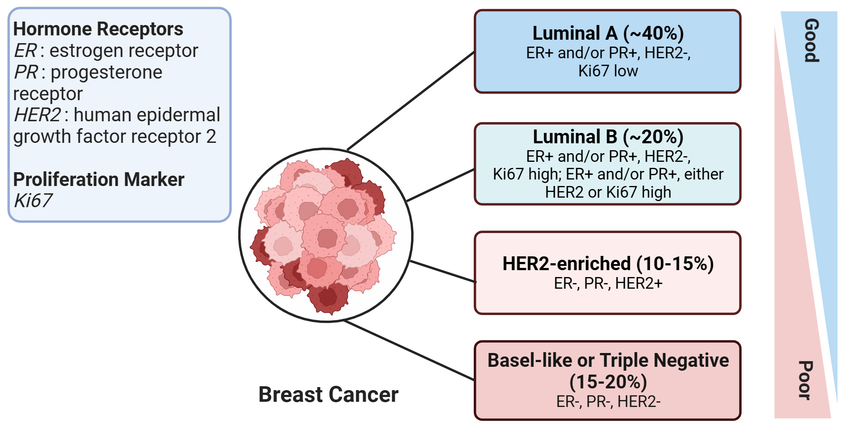
\includegraphics[width=0.8\linewidth]{reports/assets/subtypes.png}
	\caption[Classification of breast cancer molecular subtypes.]{Classification of breast cancer molecular subtypes, showing approximate proportions (\%) among all breast cancer cases. Subtypes are ordered by prognosis severity, with those having better outcomes at the top and progressively worse prognoses toward the bottom \cite{harnessing_2024}.}
	\label{fig:subtypes}
\end{figure}

In recent years, advances in artificial intelligence (AI), together with the increasing availability of data and increasingly powerful computational resources, have driven the development of deep learning (DL) models for breast cancer classification, detection, and prognosis prediction, as well as applications in other diseases. Several studies have demonstrated that these systems can match or even surpass the performance of human experts or CAD\footnote{Computer-Aided Diagnosis} systems in these tasks \cite{mckinney_international_2020,pattanaik_breast_2022,meenalochini_deep_2024,hussain_performance_2025}, highlighting the significant potential of this technology to improve clinical practice and patient outcomes.

Recent research has explored breast cancer molecular subtype classification from mammographic images. For example, Mota et al. (2024) \cite{mota_breast_2024} investigated this challenge, achieving a multi-class area under the curve (AUC)\footnote{A metric used in machine learning to evaluate the performance of classification models.} of 60.62\% using a ResNet-101 architecture. Similarly, Rabah et al. (2025) \cite{ben_rabah_multimodal_2025} obtained an AUC of 61.3\% with a Xception model in unimodal\footnote{Use only one type of data as input (images, text, video, etc.).} settings and developed a multimodal approach integrating clinical metadata, which achieved 88.87\% AUC. While unimodal approaches yield modest performance that remains below clinically acceptable thresholds (~80\% AUC), these studies highlight the diagnostic potential of mammographic imaging and underscore the importance of continued research to improve the accuracy and clinical utility of these models.

This study proposes a unimodal approach based exclusively on the inference based on mammograms from the public CMMD dataset (The Chinese Mammography Database) \cite{cai_online_2023}, comparing the performance of state-of-the-art Transformer architectures including Vision Transformer (ViT), Swin Transformer (Swin), and Multi-Axis Vision Transformer (MaxViT) against a traditional ResNet-101 baseline. While multimodal models typically achieve superior results by integrating complementary clinical data, a unimodal approach focused exclusively on mammographic images offers significant practical advantages, especially in resource-limited settings or when clinical data standardization is unavailable. Recent studies have demonstrated that Transformers-based models outperform convolutional neural networks (CNN) in accuracy and robustness for medical image classification tasks due to their self-attention mechanisms, which enable them to capture global spatial relationships across images \cite{mauricio_comparing_2023}. Based on these architectural advantages, this study hypothesizes that Transformer architectures will achieve superior performance in molecular subtype classification, even under a unimodal approach.

Ultimately, this work seeks to contribute to the development of non-invasive diagnostic tools through systematic evaluation of transformer-based models, advancing automated, accessible, and efficient molecular characterization of breast cancer. This approach is particularly valuable in clinical scenarios where tissue biopsy is not immediately feasible, potentially improving diagnostic equity and reducing time to treatment initiation.


\section{Planning}

\subsection{Objectives}

The \textbf{primary objective} of this study is to systematically compare Transformer-based architectures against a CNN baseline for mammography-based molecular subtype classification, establishing performance benchmarks for non-invasive breast cancer characterization.

To achieve this primary objective, the following \textbf{secondary objectives} are proposed:

\begin{enumerate}
	\item \textbf{Conduct a comprehensive literature review} of AI approaches for breast cancer molecular subtype classification, analyzing current research and performance benchmarks.
	\item \textbf{Identify and address dataset challenges} through appropriate preprocessing strategies, including class imbalance mitigation via weighted loss functions, balanced sampling techniques, and data augmentation methods.
	\item \textbf{Develop and implement} a robust stratified k-fold cross-validation framework for training and evaluating Vision Transformer architectures (ViT, Swin Transformer, and MaxViT) on mammographic images.
	\item \textbf{Establish comparative performance analysis} against a ResNet-101 baseline and benchmark results from existing literature using standardized evaluation metrics (Accuracy, AUC, F1-Score, Precision, Recall, Cohen-Kappa).
	\item \textbf{Perform statistical validation} of model performance differences through statistical tests to ensure result significance and reliability.
	\item \textbf{Apply interpretability analysis} using Grad-CAM and attention visualization techniques to identify mammographic features most relevant to molecular subtype discrimination.
	\item \textbf{Synthesize findings and provide recommendations} for future research directions and clinical implementation considerations.
\end{enumerate}

\subsection{Tasks to Develop}

In order to address the aforementioned objectives of the project, several tasks have been identified, as described below. 

\textbf{State of the Art}

\begin{enumerate}
	\item \textbf{Medical context}: Review current scientific literature on breast cancer to contextualize its clinical and epidemiological relevance.
	\item \textbf{Problem intuition}: Analyze the importance of molecular characterization in breast cancer, highlighting its advantages, limitations, and current challenges.
	\item \textbf{Previous works}: Examine recent advances in AI and DL for breast cancer characterization and diagnosis, comparing approaches and results reported in the literature.
\end{enumerate}

\textbf{Implementation}

\begin{enumerate}
	\item \textbf{Data Collection}: Acquire images and familiarize with the dataset's structure, organization, and provided metadata.
	\item \textbf{Data Analysis and Preprocessing}: Analyze class distribution, data consistency, and perform image preprocessing.
	\item \textbf{Project Coding}: Develop code to conduct experiments, train, and evaluate the different models.
	\item \textbf{Result Analysis}: Evaluate and interpret results to draw conclusions and propose future work.
\end{enumerate}

\textbf{Report Preparation}

\begin{enumerate}
	\item \textbf{Report Writing}: Document all procedures, including methodology, materials, results, and conclusions.
	\item \textbf{Revisions}: Incorporate feedback from advisor and refine until achieving acceptable quality.
	\item \textbf{Submission and Presentation}: Submit the thesis and prepare a summary of key findings for the committee presentation.
\end{enumerate}

\subsection{Planning}

The project planning is represented in the Gantt chart below (Figure \ref{fig:roadmap}), outlining previously defined tasks across the 4 months of the project (Spring Semester).

\begin{figure}[h!]
	\centering
	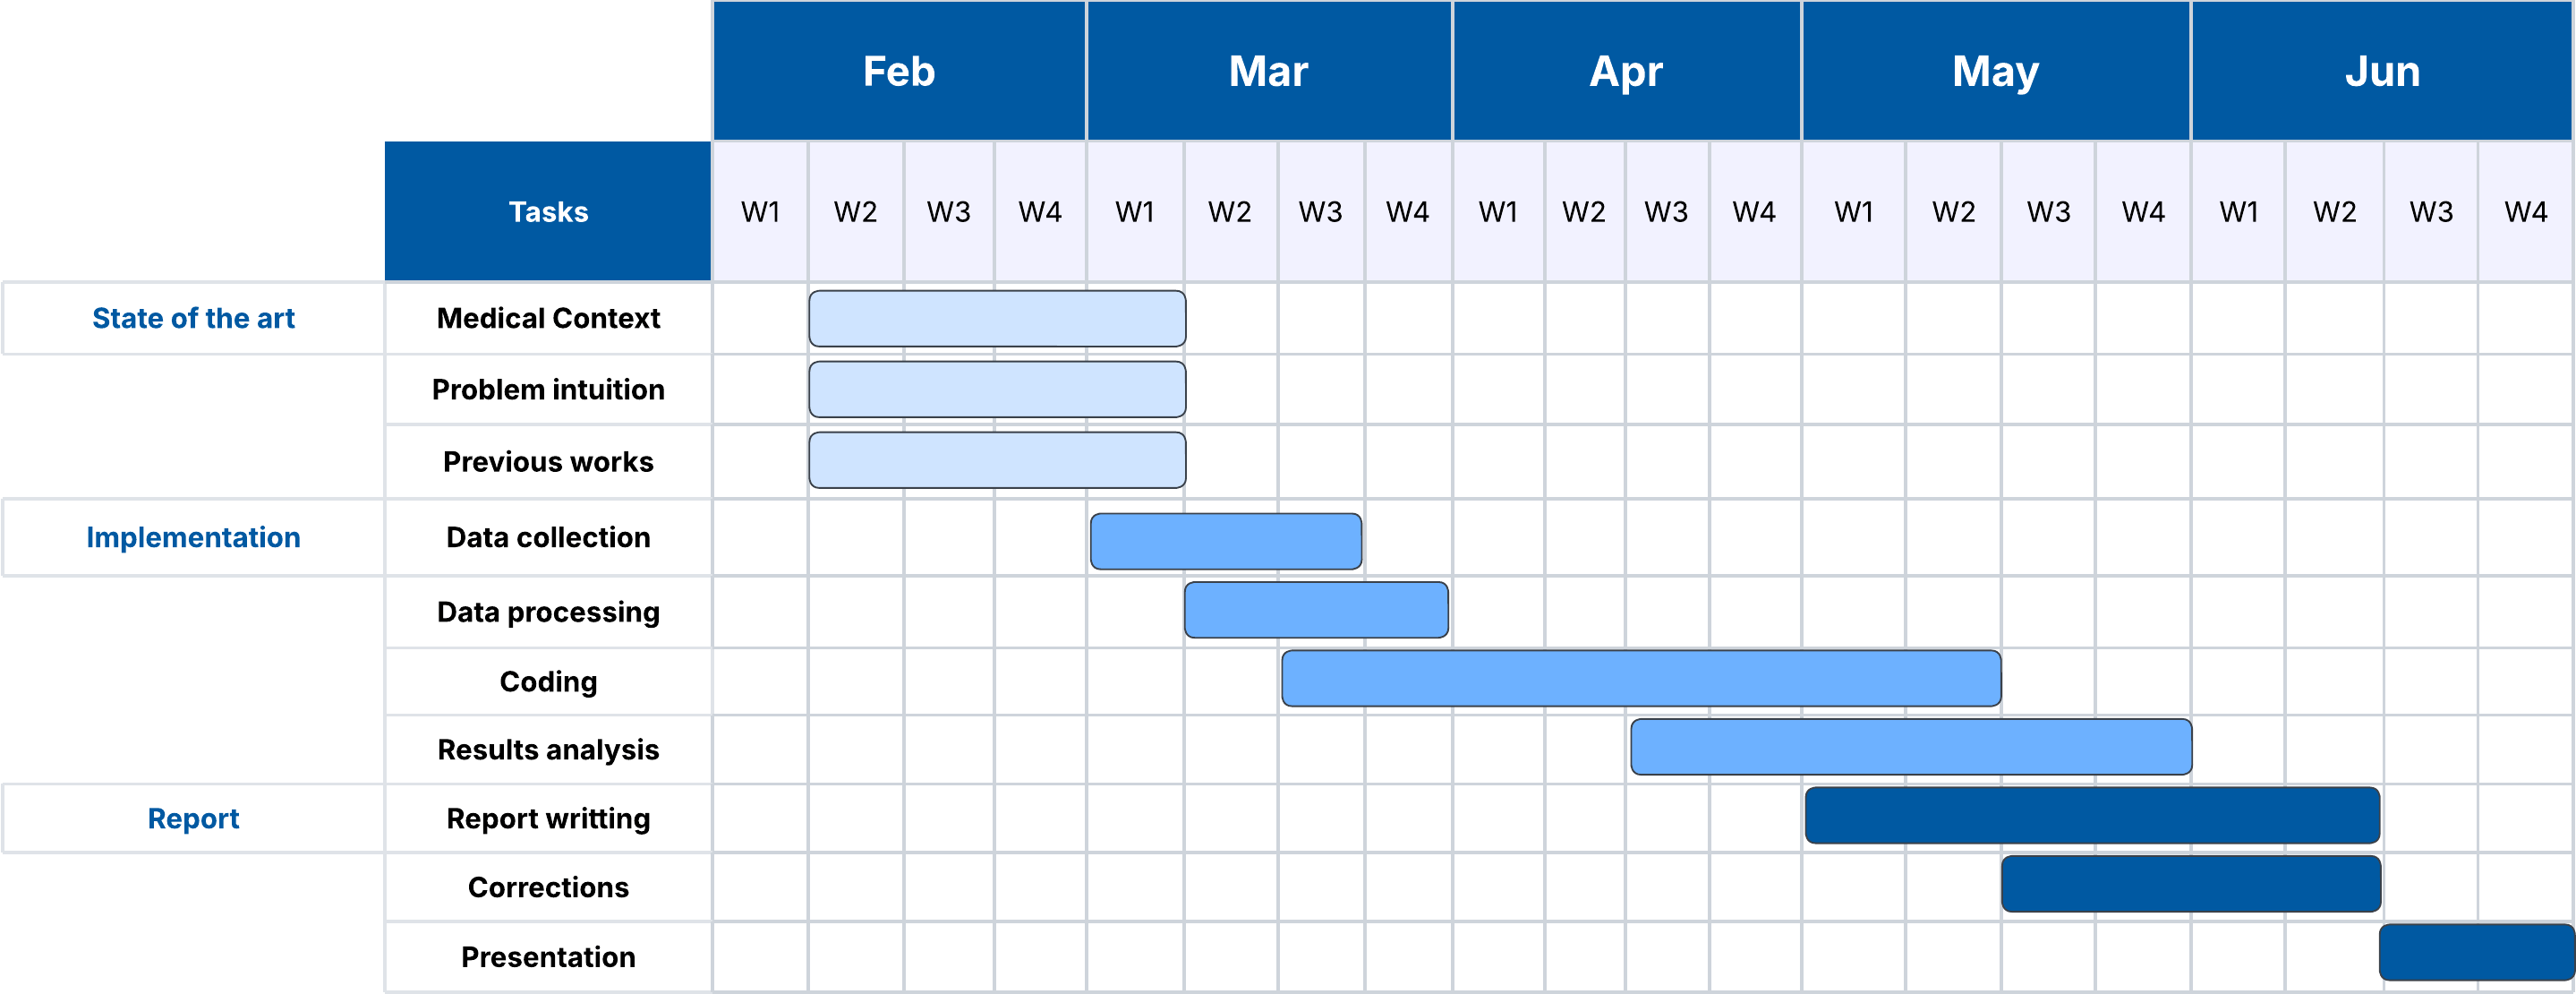
\includegraphics[width=1\linewidth]{reports//assets/RoadmapV3.png}
	\caption[Planning Gantt Chart]{Gantt Chart.}
	\label{fig:roadmap}
\end{figure}

%%%%%%%%%%%%%%%%%%%%%%%%%%%%%%%%%%%%%%%%%%%%%%%%%%%%%%%%%%%%%%%%%%%%%%%%%

\chapter{Background}

\section{Breast Cancer}

Breast cancer is a malignant neoplasm\footnote{An abnormal and uncontrolled growth of cells that gives rise to a mass or tumor, called benign if it grows slowly and remains localized, or malignant if it is invasive and fast-growing.} that originates in the glandular tissue of the breast, mainly in the ducts and lobules, where certain cells undergo genetic mutations that disrupt their growth control. 

These alterations allow cells to multiply uncontrollably, forming tumor masses that can infiltrate adjacent tissues and even spread to distant organs through the lymphatic system and bloodstream. In the absence of early diagnosis and timely treatment, this spread, also known as metastasis, can seriously compromise patient survival. Figure \ref{fig:breast-cancer-anatomy} illustrates the anatomical structure of the breast, showing how tumors develop within normal breast tissue.

\begin{figure}[h]
	\centering
	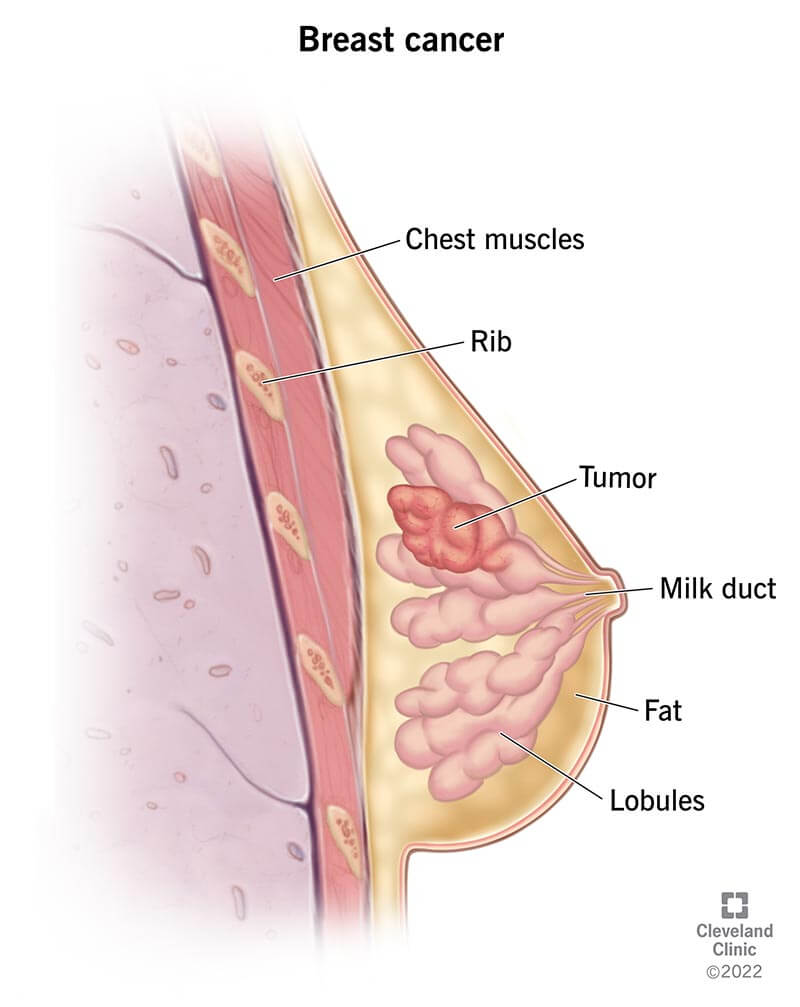
\includegraphics[width=0.3\linewidth]{reports//assets/bc.jpg}
	\caption[Anatomy of breast cancer]{Anatomy of breast cancer \cite{cleveland_clinic_breast_2023}.}
	\label{fig:breast-cancer-anatomy}
\end{figure}

\subsection{Epidemiology}

Globally, it is the most common neoplasm among women and the leading cause of cancer-related mortality in this population. In 2022, approximately 2.3 million new cases were estimated, with 670,000 deaths from this disease, according to the World Health Organization (WHO) \cite{who_breast_2024}. In Spain, breast cancer accounts for nearly 30\% of all cancer cases, and projections from the Spanish Society of Medical Oncology (SEOM) estimate around 37,400 new cases in 2025 \cite{seom_cancer_nodate}.

\subsection{Clinical Classification}

Most breast cancers are carcinomas, which are malignant tumors that originate in the ducts or lobules of the breast. These carcinomas constitute more than 95\% of all breast cancer cases \cite{makki_diversity_2015, noauthor_types_nodate}. From a clinical perspective, these tumors can be classified according to various criteria, among which the following stand out:

\textbf{According to their degree of invasion}
\begin{itemize}
	\item \textbf{Carcinoma in situ}: A tumor in which abnormal cells are confined within the breast ducts and have not crossed the natural barrier separating them from the rest of the breast tissue. Although not invasive, it is considered a precursor lesion and high-risk.
	\item \textbf{Invasive carcinoma}: A tumor that has breached the ducts or lobules of the breast and invaded the surrounding breast tissue. It can spread to lymph nodes or distant sites. 
\end{itemize}

\textbf{According to histological origin}
\begin{itemize}
	\item \textbf{Ductal carcinoma}: Originates in the milk ducts\footnote{Ducts that carry milk from the mammary glands to the nipple.} and is the most common subtype.
	\item \textbf{Lobular carcinoma}: Originates in the breast lobules and tends to show a more diffuse pattern of spread.
\end{itemize}

Figures \ref{fig:histological_types_one} and \ref{fig:histological_types_two} show the differences between ductal and lobular carcinoma, both in situ and invasive.

\begin{figure}[h!]
	\centering
	\begin{subfigure}[c]{0.48\textwidth}
		\centering
		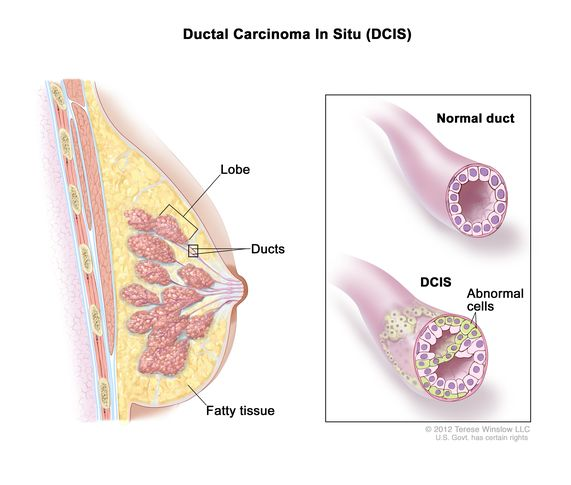
\includegraphics[width=\textwidth]{reports/assets/dcis.jpg}
		\caption{Ductal carcinoma in situ}
		\label{fig:dcis}
	\end{subfigure}
	\begin{subfigure}[c]{0.48\textwidth}
		\centering
		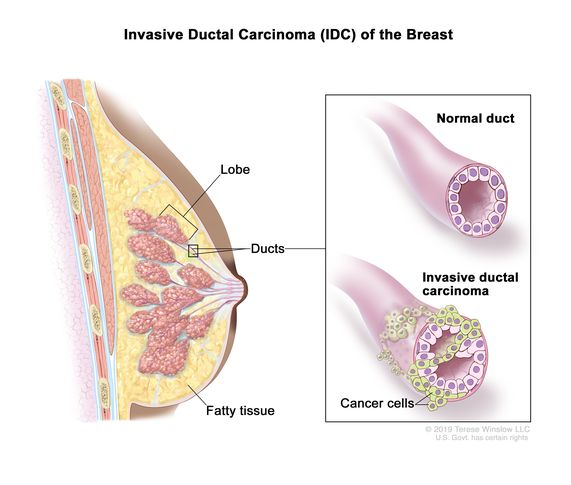
\includegraphics[width=\textwidth]{reports/assets/idc.jpg}
		\caption{Invasive ductal carcinoma}
		\label{fig:idc}
	\end{subfigure}
	\caption[DCIS vs. IDC comparison]{Anatomical comparison between ductal carcinoma in situ (DCIS) and invasive ductal carcinoma (IDC). (a) DCIS shows abnormal cells confined within the milk duct structure, while (b) IDC demonstrates cancer cells that have broken through the duct wall and invaded surrounding breast tissue \cite{noauthor_nci_2011}.}
	\label{fig:histological_types_one}
\end{figure}

\begin{figure}[h!]
	\centering
	\begin{subfigure}[c]{0.48\textwidth}
		\centering
		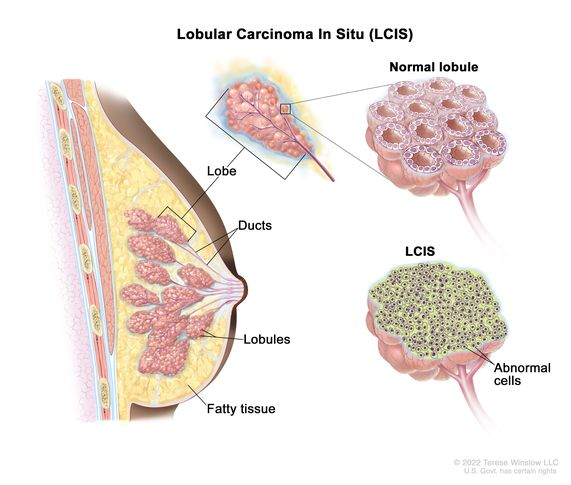
\includegraphics[width=\textwidth]{reports/assets/lcis.jpg}
		\caption{Lobular carcinoma in situ}
		\label{fig:lcis}
	\end{subfigure}
	\begin{subfigure}[c]{0.48\textwidth}
		\centering
		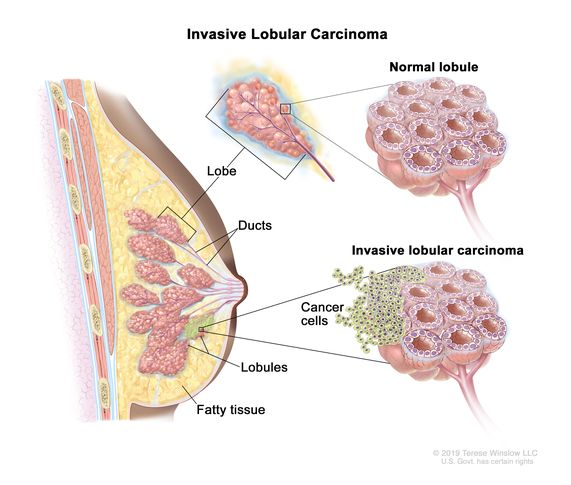
\includegraphics[width=\textwidth]{reports/assets/ilc.jpg}
		\caption{Invasive lobular carcinoma}
		\label{fig:ilc}
	\end{subfigure}
	\caption[LCIS vs. ILC comparison]{Progression from lobular carcinoma in situ (LCIS) to invasive lobular carcinoma (ILC). (a) LCIS represents abnormal cell growth restricted to the milk-producing lobules, whereas (b) ILC shows malignant cells spreading from lobules into adjacent breast tissue \cite{noauthor_nci_2011}.}
\label{fig:histological_types_two}
\end{figure}

\textbf{According to staging systems}

Clinical staging systems are a way of determining how much cancer there is and how far it has spread in the body, using tests and assessments done before surgery or other treatment. This provides standardized frameworks for prognosis and treatment planning.

\begin{itemize}
	\item \textbf{BI-RADS Staging System}: The Breast Imaging-Reporting and Data System (BI-RADS)\cite{magny_breast_2025} standardizes mammographic interpretation and assigns suspicion categories that guide medical management (see Table \ref{tab:birads_table}).
    \item  \textbf{TNM Staging System}: This is the most widely used staging system \cite{noauthor_stages_nodate}. It evaluates three key anatomical factors:
    \begin{itemize}
        \item \textbf{Tumor(T)}: Size and local extent of the primary tumor, ranging from TX (tumor cannot be assessed) to T4 (extensive local invasion).
        \item \textbf{Node(N)}: Regional lymph node involvement, from NX (nearby lymph nodes cannot be assessed) to N3 (extensive nodal spread).
        \item \textbf{Metastasis(M)}: Presence or absence of distant metastases (M0 or M1).
  \end{itemize}
  The current TNM system, updated in 2018, incorporates new parameters like estrogen receptor (ER), progesterone receptor (PR), and others clinical variables to provide more accurate prognostic stratification \cite{hortobagyi_new_2018}. 
  
\end{itemize}

\begin{table}[h!]
	\caption[Breast Imaging-Reporting and Data System (BI-RADS)]{Breast Imaging-Reporting and Data System (BI-RADS) classification \cite{noauthor_bi-rads_2025}.}
	\centering
	\begin{tabular}{lccccc}
		\toprule
		\textbf{Category} & \textbf{Definition} & \textbf{Likelihood of cancer}\\
		\midrule
		BI-RADS 0        & Incomplete                         & N/A \\
		BI-RADS 1        & Negative                           & Essentially 0\% \\
            BI-RADS 2        & Benign                             & Essentially 0\%  \\
            BI-RADS 3        & Probably benign                    & > 0\% but $\leq 2\%$ \\
            BI-RADS 4        & Suspicious                         & > 2\% but < 95 \% \\
            BI-RADS 5        & Highly suggestive of malignancy    & $\geq 95\%$ \\
            BI-RADS 6        & Known biopsy-proven malignancy     & N/A \\
		\bottomrule
	\end{tabular}
	\label{tab:birads_table}
\end{table}


In addition to these classifications, in recent years, molecular subtyping of breast cancer, based on biomarker expression and genomic profiles, has gained particular relevance, which will be addressed in the next section.


\subsection{Molecular Subtypes}

Although clinical and histological classification of breast cancer provides important information for diagnosis, it does not always allow for precise prediction of the tumor’s biological behavior or its response to specific treatments.

The research by Perou et al. (2000) \cite{perou_molecular_2000} and Sørli et al. (2003) \cite{sorlie_repeated_2003} laid the groundwork for the molecular characterization of breast cancer. Through gene expression profiling\footnote{A study that identifies which genes are active and to what extent in a cell or tissue by analyzing RNA levels produced by thousands of genes simultaneously.}, Perou et al. demonstrated that breast cancer is a heterogeneous disease and proposed a molecular subtype classification based on the genetic expression patterns of the tumors analyzed. Four subtypes were initially defined: \textbf{Luminal A}, \textbf{Luminal B}, \textbf{HER2}, and \textbf{Basal-like (Triple negative)}.

Sørli et al. reinforced these findings. They replicated the research in different patient cohorts, demonstrating that the results were not artifacts of a single study. They also showed that molecular subtypes are associated with clinically significant differences, such as prognosis and risk of distant metastasis, giving this characterization greater predictive value than traditional histological classification.

\begin{figure}
	\centering
	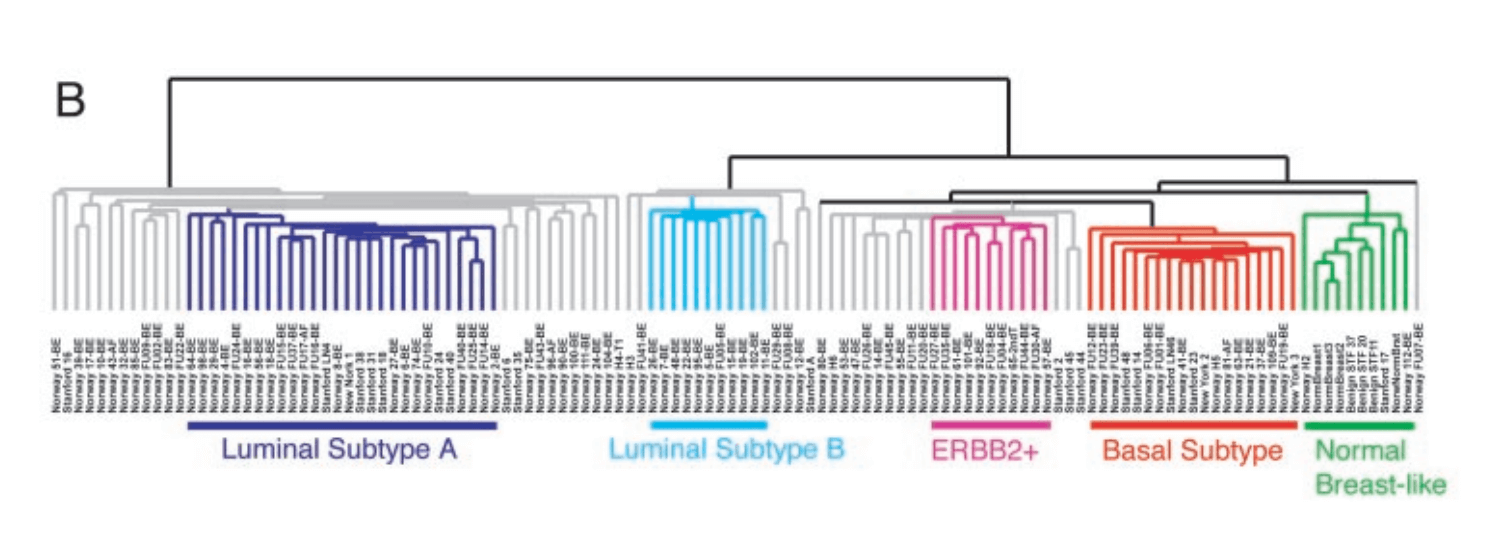
\includegraphics[width=0.8\linewidth]{reports//assets/dendogram.png}
	\caption[Molecular subtypes dendrogram by Sørli et al.]{Dendrogram from the study by Sørli et al. showing the clustering of subtypes according to genetic patterns \cite{sorlie_repeated_2003}.}
	\label{fig:sorlie-dandrogram}
\end{figure}

Following these studies, efforts focused on translating the findings into clinical practice. Since the technique used for classification at the time (DNA microarrays) was expensive, complex, and not accessible to most hospitals, an alternative was sought. It was at the St. Gallen international consensus meetings that classification criteria based on immunohistochemical (IHC) markers\footnote{Specific proteins or antigens present in cells or tissues that can be detected using antibodies in a laboratory technique called immunohistochemistry.} were proposed, formalizing the subtypes using a combination of the following hormone receptors \cite{lips_breast_2013}:

\begin{itemize}
	\item \textbf{Estrogen (ER) and Progesterone (PR) Receptors}: Define the tumor’s hormonal dependence, which can affect its growth. Tumors with these receptors respond well to hormonal therapy.
	\item \textbf{HER2 (Human epidermal growth factor receptor 2)}: A protein that stimulates cell growth. Its overexpression usually indicates a more aggressive subtype.
	\item \textbf{Ki-67}: The cell proliferation index. High Ki-67 suggests a more aggressive and rapidly proliferating tumor.
\end{itemize}

Table \ref{tab:molecular_subtypes_comb} shows these classification criteria.

\begin{table}[h!]
	\centering
        \caption[Breast cancer molecular subtypes classification criteria]{Classification criteria for molecular subtypes from the St. Gallen 2013 consensus \cite{goldhirsch_personalizing_2013}}.
	\begin{tabular}{lccccc}
		\toprule
		\textbf{Subtype} & \textbf{HER2} & \textbf{ER} & \textbf{PR} & \textbf{Ki-67} \\
		\midrule
		Luminal A        & Negative      & Positive    & Positive    & < 14\%         \\
		Luminal B/HER2-  & Negative      & Positive    & -           & $\geq$ 14\%    \\
		Luminal B/HER2+  & Positive      & Positive    & -           & -              \\
		HER2-enriched    & Positive      & Negative    & Negative    & -              \\
		Triple Negative  & Negative      & Negative    & Negative    & -              \\
		\bottomrule
	\end{tabular}
	\label{tab:molecular_subtypes_comb}
\end{table}

The Luminal A subtype is the most frequent, representing 70\% of cases at diagnosis. These tumors are characterized by slower growth and respond well to hormonal therapies, making them tumors with a better prognosis and higher survival rates. Luminal B tumors are more aggressive, have a more guarded prognosis, and are more likely to recur. They tend to be more resistant to hormonal treatments and may require chemotherapy.

HER2-enriched tumors account for 10–15\% of cases, distinguished by a rapid growth rate and overexpression of HER2, without hormone receptors. Finally, the triple negative subtype, also appearing in 10–15\% of diagnoses, lacks expression of ER, PR, and HER2. This group displays more aggressive clinical behavior, with a high rate of early recurrence and limited therapeutic options, as it does not respond to hormone therapy or targeted treatments. Conventional chemotherapy is currently the main therapeutic strategy.

\section{Medical Imaging}

Medical imaging encompasses a set of techniques and procedures used to generate visual representations of the interior of the human body for clinical and scientific purposes. These tools enable non-invasive visualization of anatomical structures and physiological processes, facilitating disease diagnosis and the study of normal and pathological anatomy.

For breast cancer diagnosis, several imaging techniques are currently employed, each with specific advantages and limitations depending on patient characteristics and clinical context, as shown in Figure \ref{fig:breast_cancer_medical}.

\begin{figure}[h!]
    \centering
    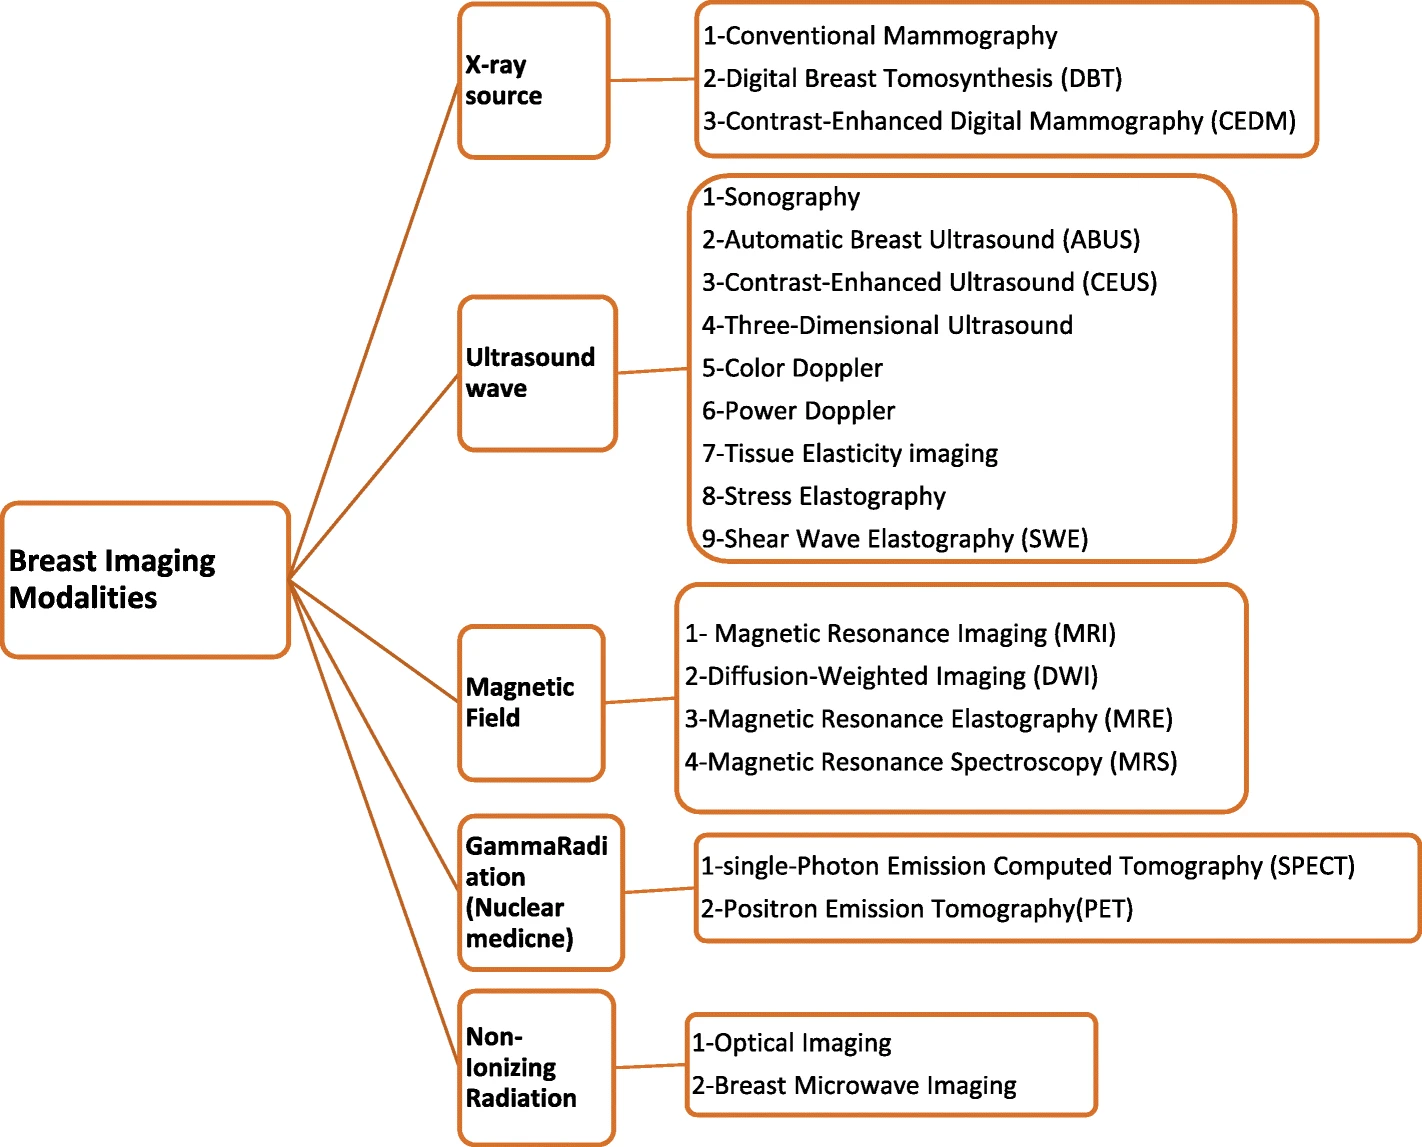
\includegraphics[width=0.75\linewidth]{reports//assets/medical_imaging.png}
    \caption[Overview of breast imaging modalities]{Overview of breast imaging modalities classified by the type of physical principle used, including x-ray, ultrasound, magnetic field, gamma radiation and non-ionizing techniques \cite{iranmakani_review_2020}.}
    \label{fig:breast_cancer_medical}
\end{figure}

\subsection{X-ray Mammography}

In this work, X-ray mammography images will be used as input to our model to infer the molecular subtype of breast cancer. As the standard imaging technique in population-based screening programs, X-ray mammography was specifically developed to examine the breast and other soft tissues. The procedure is performed using a specialized medical imaging device known as a mammography unit or mammography machine. During the exam, the breast is positioned on a flat support plate and gently compressed with a paddle. A brief burst of X-rays is then passed through the breast to a detector on the opposite side, which captures detailed images for analysis (Figure \ref{fig:mammography}).

\begin{figure}[h!]
    \centering
    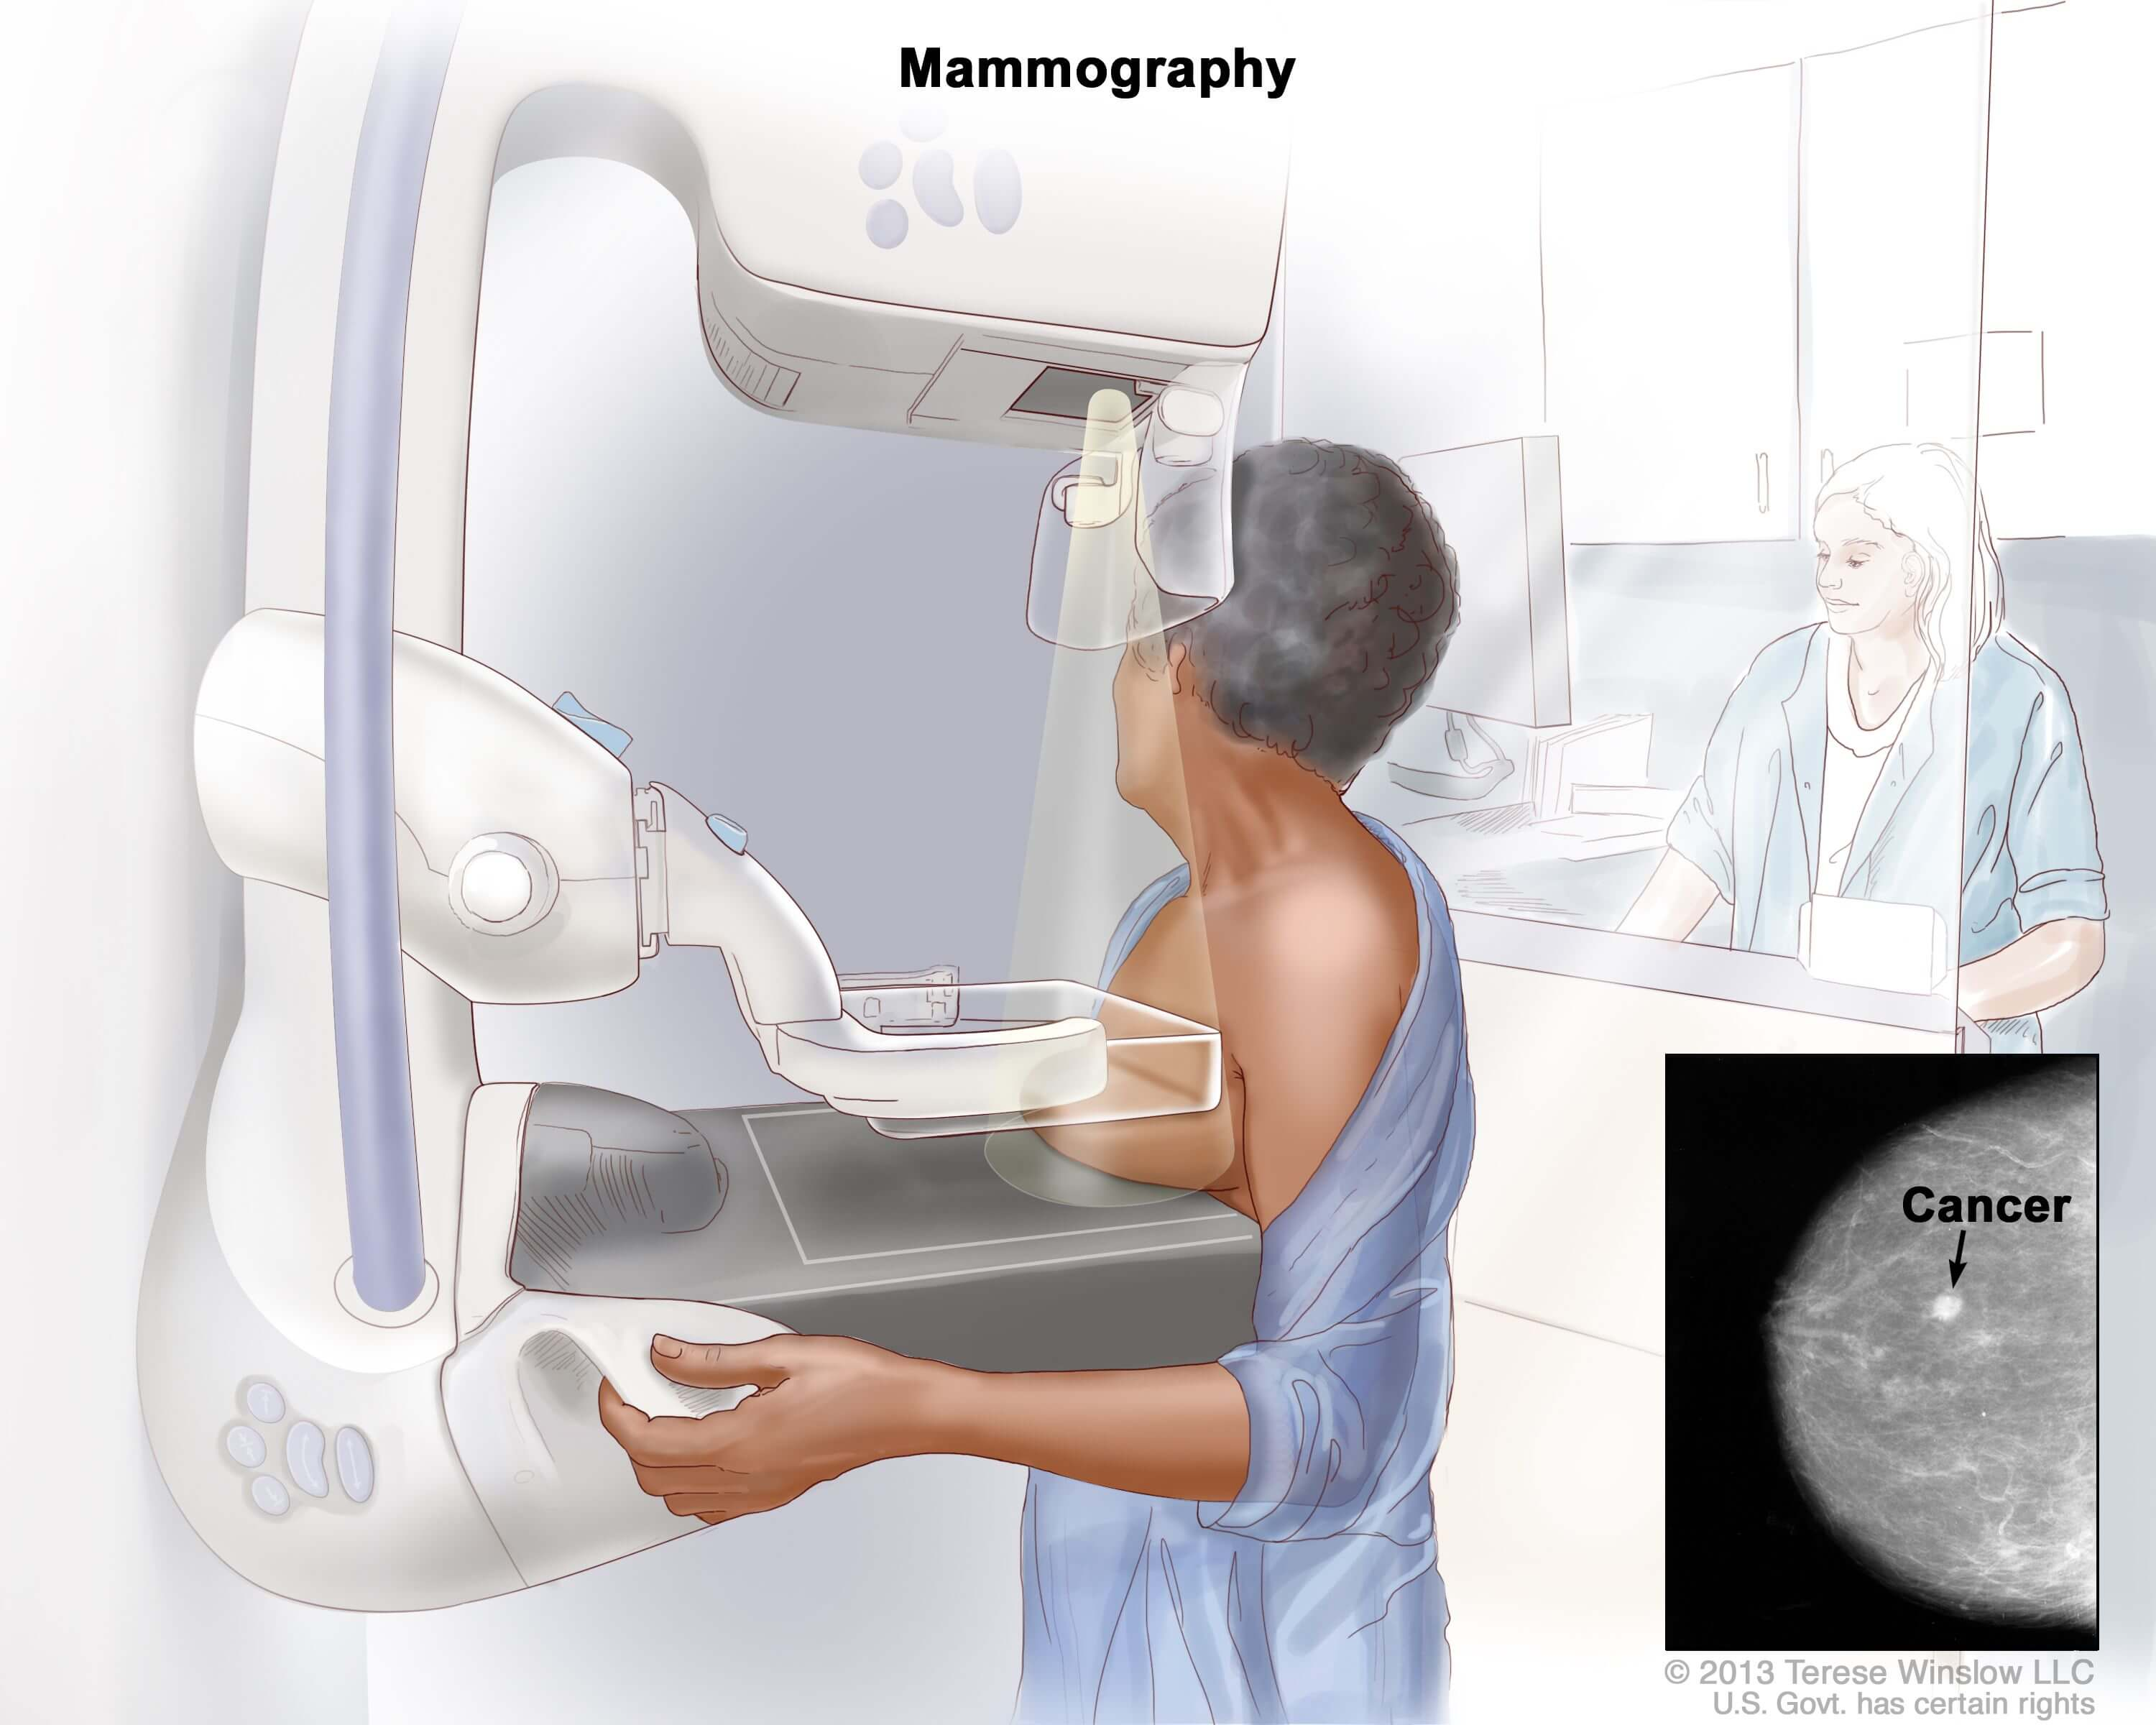
\includegraphics[width=0.45\linewidth]{reports//assets/mammography.jpg}
    \caption[Traditional mammography procedure]{Illustration showing the traditional mammography procedure \cite{nihDefinitionMammogramNCI2011}.}
    \label{fig:mammography}
\end{figure}


Each breast is typically imaged using two standard views to ensure tissue visualization:

\begin{itemize}
    \item \textbf{Craniocaudal (CC) view}: CC view is obtained from above the breast (head-to-foot) providing a top-down perspective (0º), allowing a greater visualization of the posterior and superior breast tissue. This view is particular effective for identifying whether abnormalities are located medial or lateral to the nipple \cite{noauthor_guide_nodate}.
    \item \textbf{Mediolateral oblique (MLO) view}: In the MLO view, the breast is compressed at an oblique angle (usually around 45º), enabling coverage of nearly all breast tissue \cite{noauthor_guide_nodate}. This view is particularly valuable because it includes the axillary tail and a significant portion of the pectoralis major muscle, areas where a considerable percentage (between 30\% and 40\%) of breast cancer are found \cite{aljarrah_trends_2014, noauthor_breast_2015}.
\end{itemize}



\begin{figure}[h!]
    \centering
    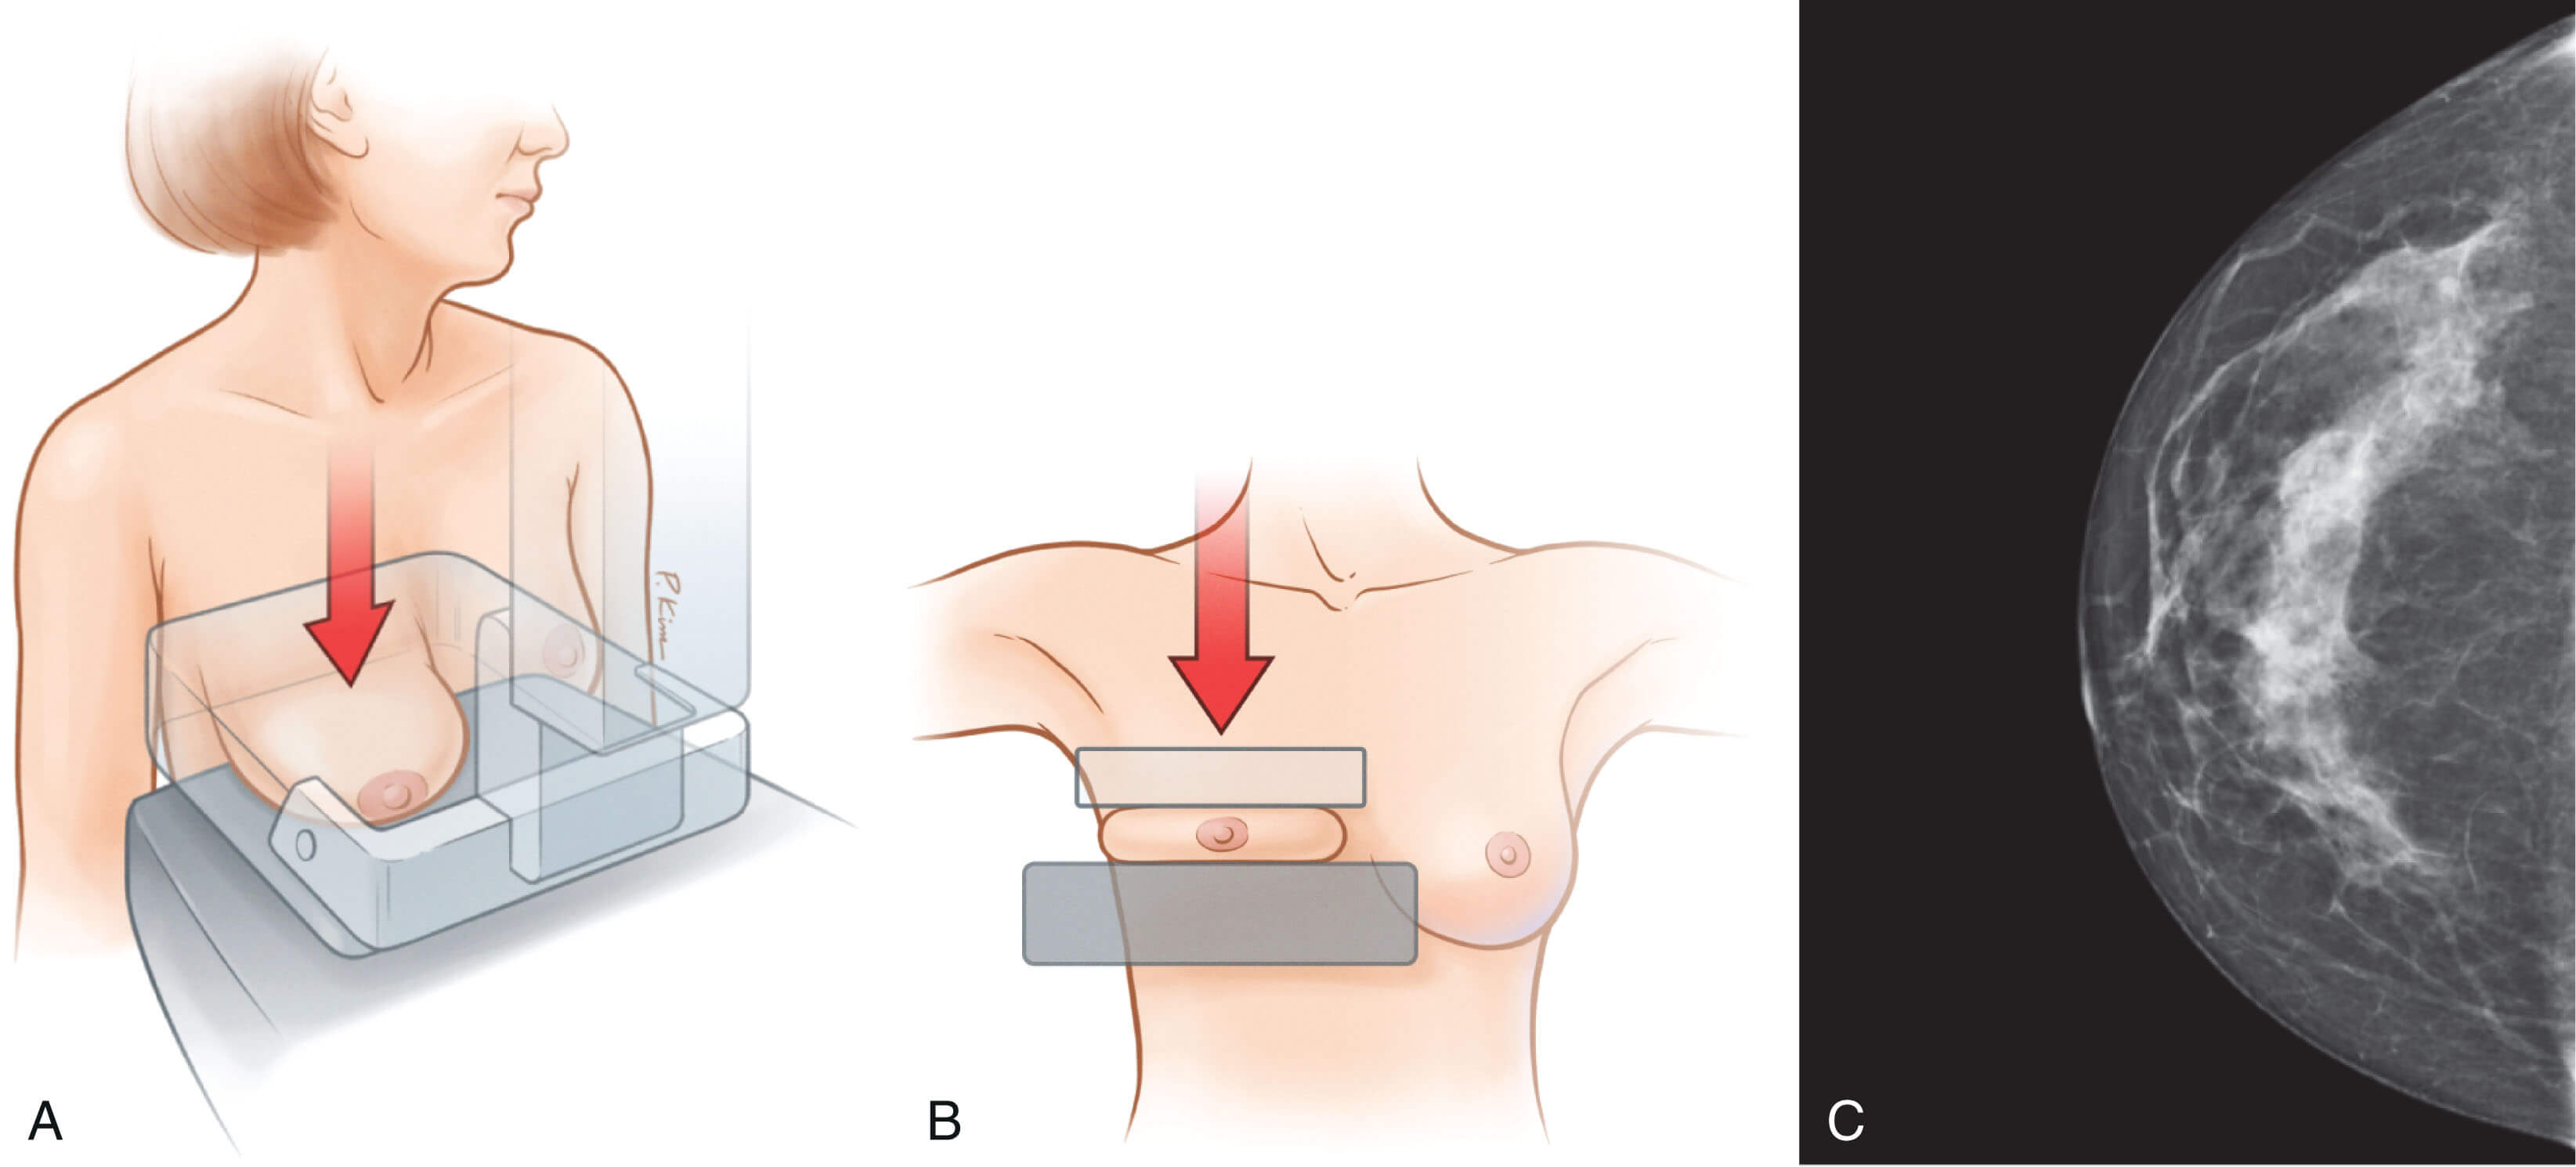
\includegraphics[width=0.6\linewidth]{reports//assets/cc_view.jpg}
    \caption[CC view acquisition procedure]{Illustration of CC view acquisition: (a) The breast is positioned horizontally on the detector and compressed with a paddle. (b) Top-down compression is applied to obtain the X-ray projection. 
    (c) Resulting mammogram image (CC view) \cite{imaging_introduction_2022}. }
    \label{fig:cc_view}
\end{figure}

\begin{figure}[h!]
    \centering
    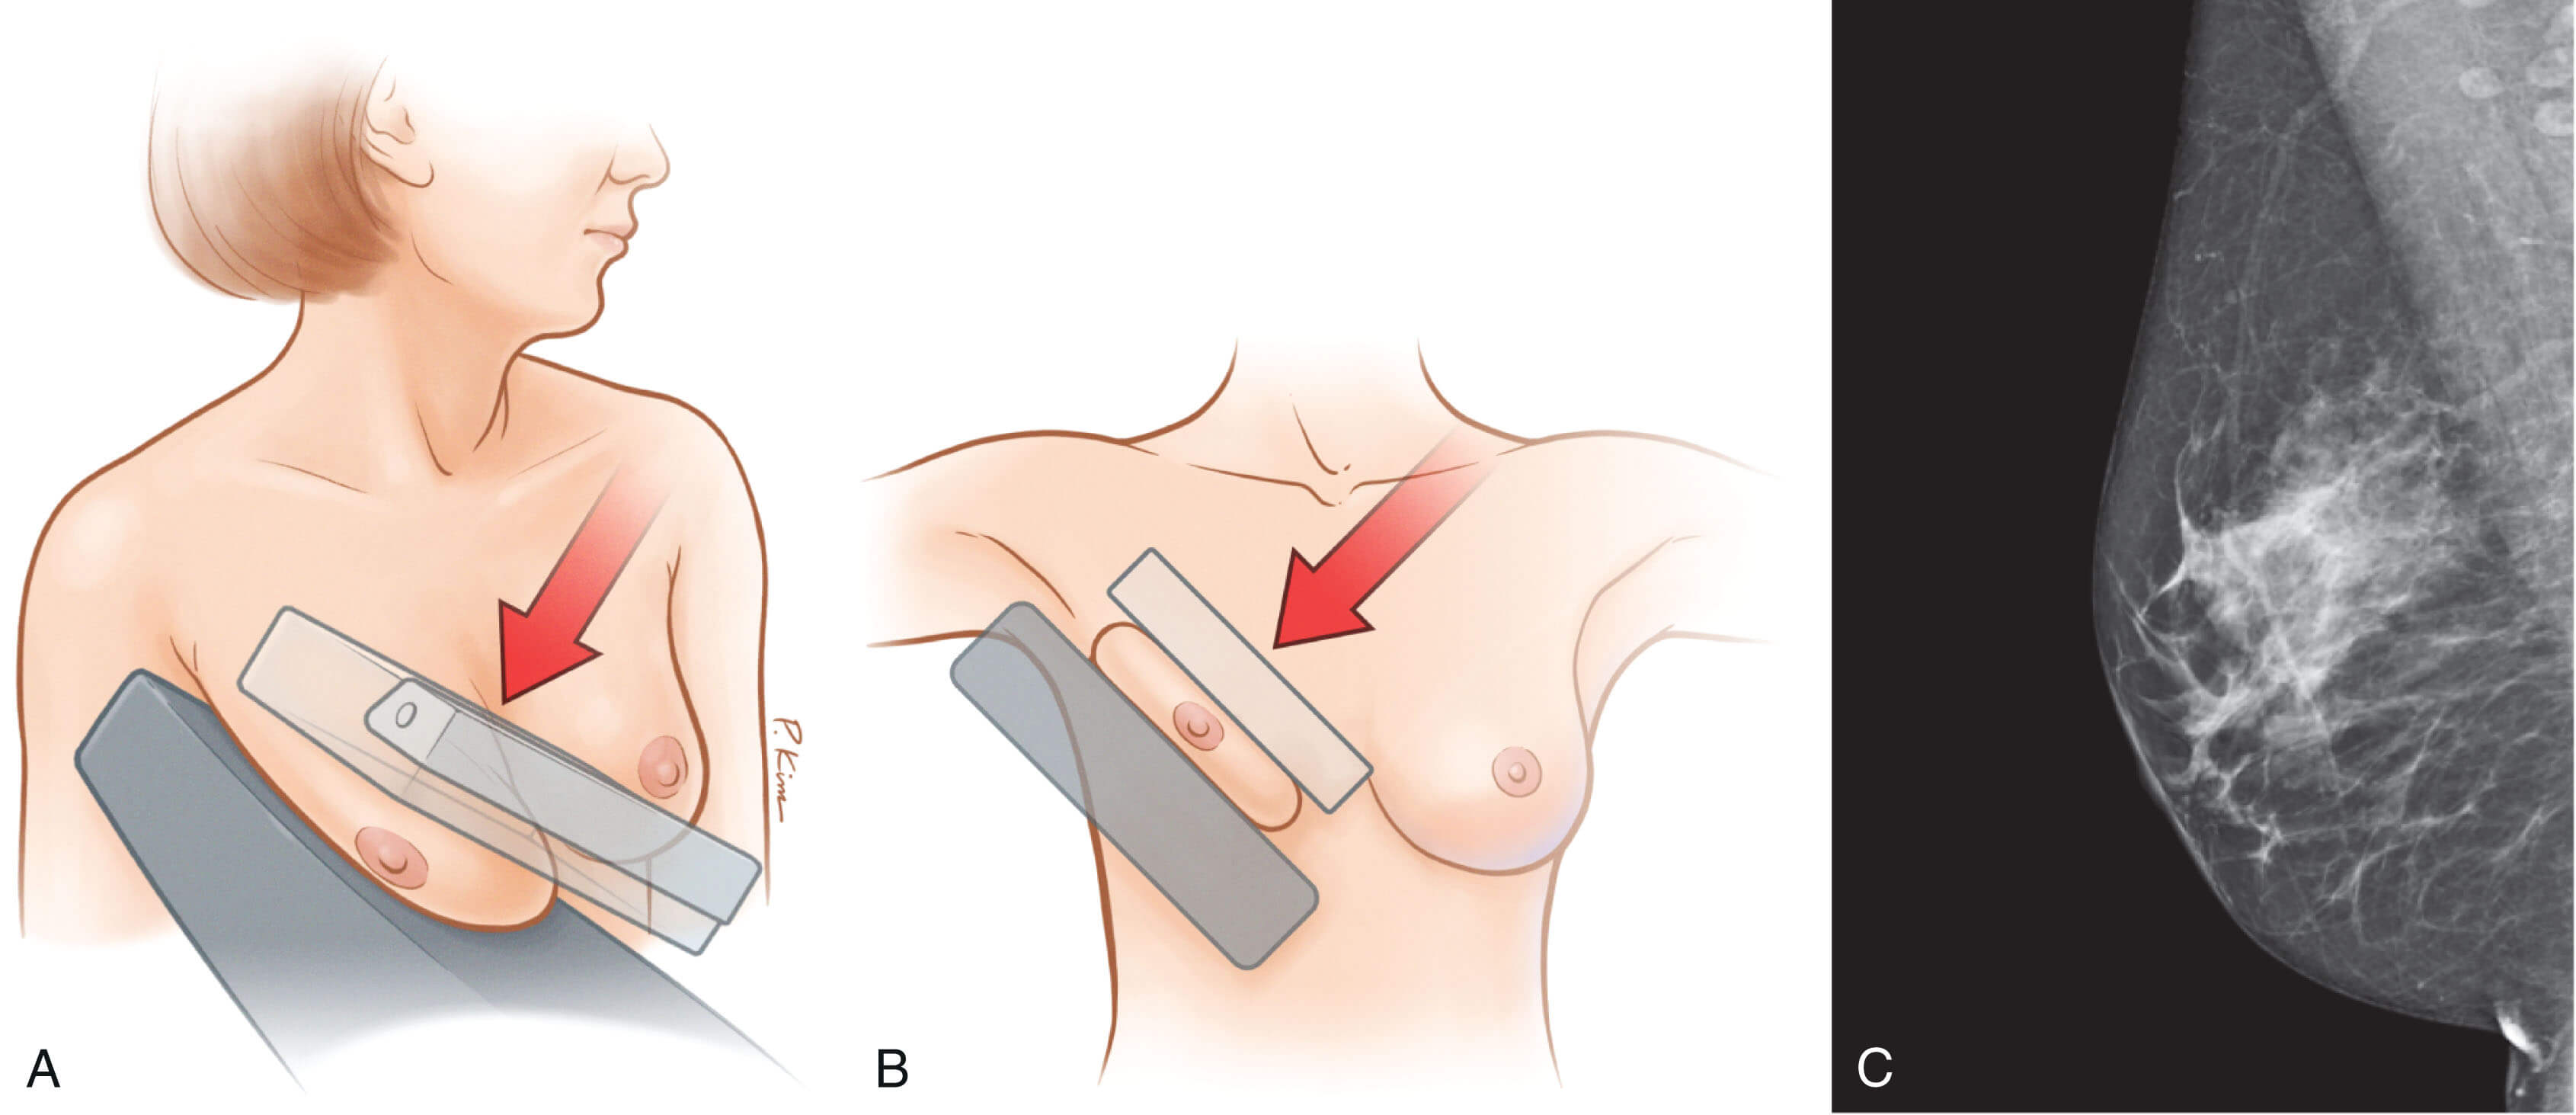
\includegraphics[width=0.6\linewidth]{reports//assets/mlo_view.jpg}
    \caption[MLO view acquisition procedure]{Illustration of MLO view acquisition: (a) The breast is positioned at an oblique angle on the detector and compressed with a paddle. (b) Compression is applied from the upper inner to the lower outer aspect to obtain the oblique X-ray projection. c) Resulting mammogram image (MLO view) \cite{imaging_introduction_2022}.}
    \label{fig:mlo_view}
\end{figure}


Modern mammography units can be either analog or digital, with digital mammography now representing the most widely used and preferred technology in clinical practice \cite{ltd_mammography_2025, noauthor_mammography_nodate}. Digital systems offer significant advantages over their analog counterparts, including immediate image acquisition, enhanced image quality, and easier storage and retrieval.

These technological advancements have further strengthened the role of mammography in clinical care. The use of x-ray mammography enables the identification of breast cancers, benign tumors, and cysts before they become palpable, often detecting tumors at a much earlier stage than physical examination alone \cite{staff_what_2025}. As a result, this technique is employed not only for routine screening in asymptomatic women, but also for diagnosing breast cancer following the detection of a lump or other symptoms, as well as for ongoing surveillance after a breast cancer diagnosis.

\subsection{Other modalities}

\textbf{Breast Ultrasound}

Breast ultrasound imaging is a widely used technique for breast analysis that uses a handheld device called a transducer\footnote{A device that produces sound waves that bounce off body tissues, receives the echoes, and transforms the signals into pictures.} to produce real-time images of the internal breast tissue by emitting high-frequency sound waves (Figure~\ref{fig:breast_ultrasound_comparison}).

Unlike mammography, ultrasound does not use ionizing radiation, making it a safe and non-invasive option for patients of all ages. This modality is particularly valuable for evaluating palpable lumps, distinguishing between solid and cystic masses, and further characterizing lesions detected on mammography, especially in women with dense breast tissue, where mammography may be less sensitive \cite{gokhale_ultrasound_2009}.

However, it is important to take into consideration that the accuracy and quality of ultrasound examinations are highly dependent on the skill and experience of the operator. In addition, compared to mammography, ultrasound is less effective at distinguishing between benign and malignant lesions, which may result in more follow-up procedures.

\begin{figure}[h!]
	\centering
	\begin{subfigure}[c]{0.45\textwidth}
		\centering
		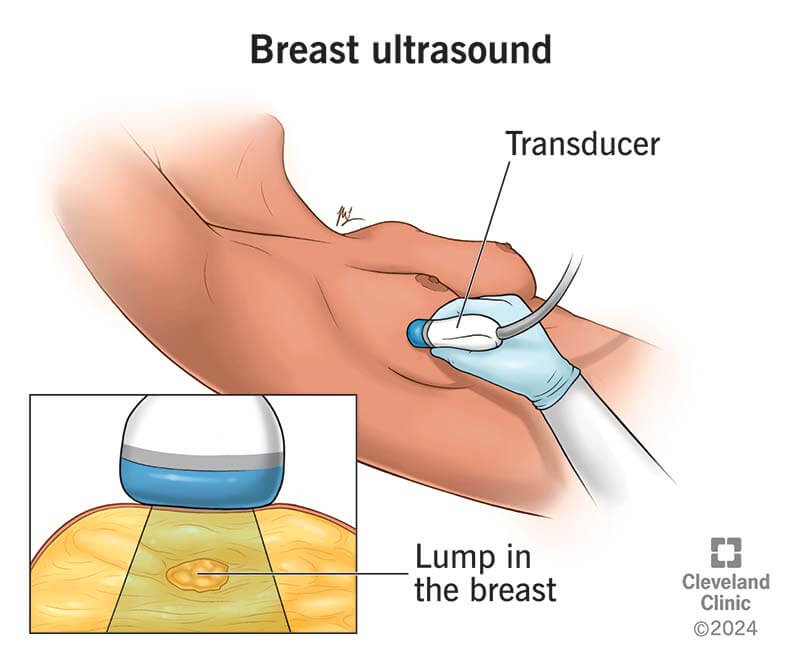
\includegraphics[width=\textwidth]{reports/assets/breast_ultrasound.jpg}
            \caption{}
		\label{fig:breast_ultrasound}
	\end{subfigure}
	\begin{subfigure}[c]{0.45\textwidth}
		\centering
		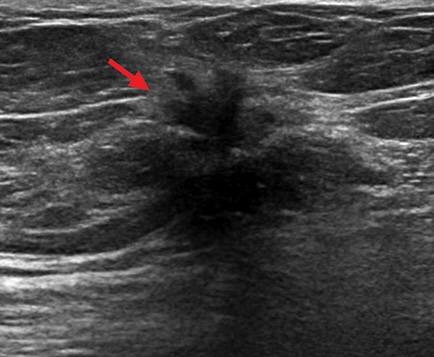
\includegraphics[width=\textwidth]{reports/assets/ultrasound.jpg}
            \caption{}
		\label{fig:ultrasound}
	\end{subfigure}
	\caption[Breast ultrasound procedure and example]{(a) Breast ultrasound representation \cite{macauley_start--finish_2022}. (b) Breast ultrasound example showing an irregular, dark gray spiculated mass, highly suspicious for cancer \cite{noauthor_breast_nodate}.}
\label{fig:breast_ultrasound_comparison}
\end{figure}

\textbf{Magnetic Resonance Imaging (MRI)}

MRI is a noninvasive imaging procedure that uses strong magnetic fields and radio waves to produce a series of highly detailed images of structures inside the body. In breast imaging, MRI operates on the same fundamental principle and is often used alongside other breast imaging modalities to detect breast cancer or other abnormalities \cite{nih_definition_2011}. 

Breast MRI is particularly valuable for women at high risk of developing breast cancer, such as those with genetic mutations or a strong family history of the disease. This is due to its high sensitivity, with detection rates exceeding 90\%, making it the most sensitive imaging modality for identifying breast cancer \cite{radswiki_breast_nodate}.

Despite these advantages, MRI is more expensive and less widely available than mammography or ultrasound. Its high sensitivity can sometimes lead to more false positives, resulting in additional follow-up imaging. Furthermore, accurate interpretation of breast MRI requires specialized training and experience \cite{noauthor_technical_nodate}.


\begin{figure}
    \centering
    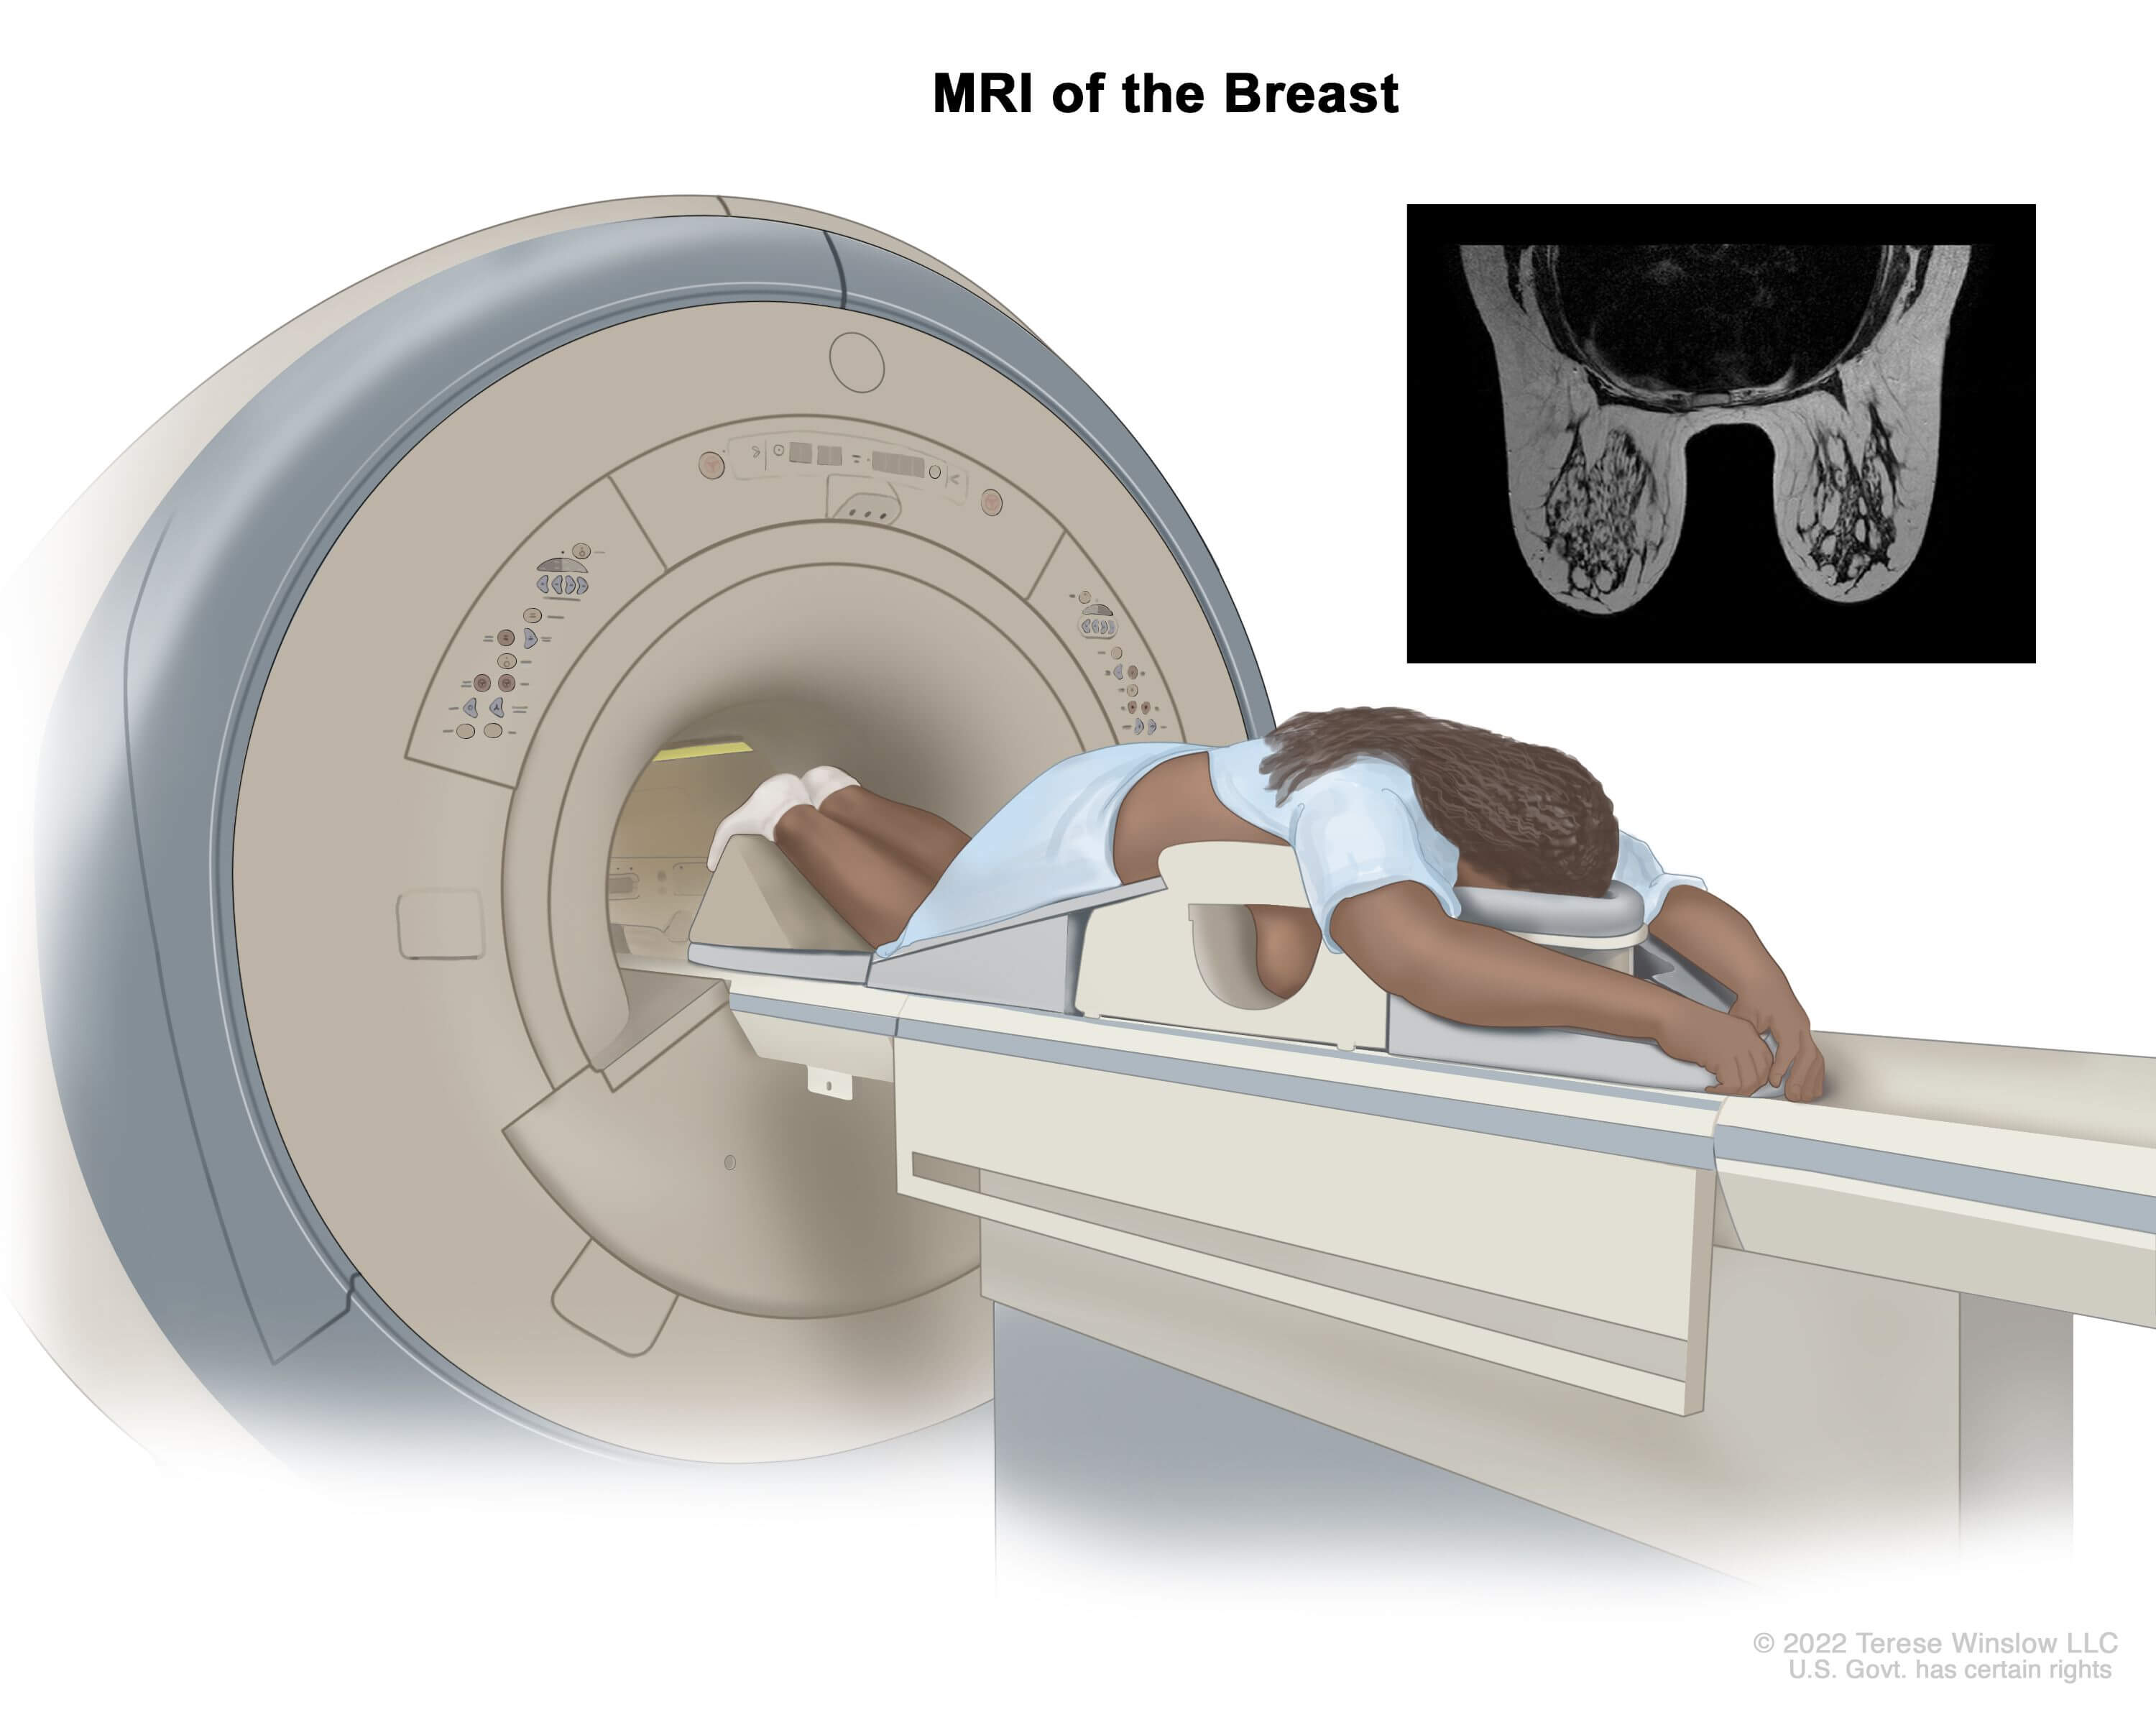
\includegraphics[width=0.5\linewidth]{reports//assets/breast_mri.jpg}
    \caption[Breast MRI procedure]{Illustration of a breast MRI procedure. The patient lies prone on a dedicated breast coil, allowing for optimal imaging of the breast tissue \cite{nih_definition_2011}.}
    \label{fig:breast_mri}
\end{figure}


\section{Cancer Screening}

Cancer screening is the process of using tests to look for cancer or pre-cancerous changes in people, mainly targeting those who do not have any symptoms of the disease. The purpose is to detect cancer at an early stage, when treatment is more likely to be successful and before symptoms appear \cite{noauthor_cancer_2010}.

There are different kinds of screening tests that can be used in the process depending on the subject’s needs. These may include physical examinations and clinical history reviews, laboratory tests, imaging procedures, and genetic tests \cite{noauthor_cancer_2010}. In the context of breast cancer, x-ray mammography is the gold-standard screening tool. As mentioned earlier, it is a widely available, noninvasive, and cost-effective technique, and it has been proven to detect tumors up to two years before they become palpable or cause symptoms \cite{cancer_que_2023}.

\subsection{General process description}

The general process of breast screening is very similar worldwide in its main steps, but certain aspects, such as the starting age, screening frequency, and technology used may vary from country to country. In Spain, the breast cancer screening program began in 1990 and is performed only in women between 50 and 69 years old, using biennial\footnote{Every two years} mammograms \cite{noauthor_ministerio_nodate}. The following steps are the core steps of breast cancer screening:

\begin{enumerate}
    \item \textbf{Invitation}: Eligible women (based on age and sometimes risk factors) are invited to participate, either through organized national programs or through healthcare providers.
    \item \textbf{Screening test}: The screening test is performed, typically a mammogram, which may be supplemented by other tests. For example, in Spain, an ultrasound is also recommended \cite{noauthor_map_nodate}.
    \item \textbf{Image review}: Radiologists review the mammograms for signs of cancer, such as masses or microcalcifications.
    \item \textbf{Results notification}: Women are informed of their results. Those with abnormal findings are called back for additional tests.
    \item \textbf{Follow-up}: If abnormalities are detected, further diagnostic procedures, such as additional imaging or biopsy, are conducted to confirm or rule out cancer.
\end{enumerate}


At this stage, non-invasive techniques, such as those investigated in this work, can contribute to improved diagnostic outcomes and offer more detailed insights. Specifically, in the context of molecular subtype classification, having such a tool would provide additional information for cases with abnormal findings or confirmed cancers. This could lead to a better prognosis and help guide clinical decision-making, potentially reducing the need for further invasive procedures like biopsies.

\subsection{Biopsy Techniques}

When imaging or other screening tests detect abnormalities suggestive of breast cancer, a biopsy is typically required to obtain a definitive diagnosis. A breast biopsy involves removing a small sample of tissue from the suspicious area, which is then examined under a microscope by a pathologist \cite{DefinitionBiopsyNCI2011}. This step is crucial not only for confirming the presence of cancer but also for determining its type, grade, and increasingly, its molecular characteristics.

\textbf{Classification}

Several biopsy techniques are commonly used for the diagnosis and characterization of breast lesions, including:

\begin{itemize}
    \item \textbf{Fine Needle Aspiration (FNA)}: A minimally invasive procedure that uses a thin, hollow needle to extract cells or fluid from a suspicious area. It is often performed when the lesion is likely to be a cyst\footnote{A fluid-filled sac}. FNA is quick, cost-effective, and generally well-tolerated, offering high diagnostic accuracy when performed correctly. However, it may provide limited information about tissue structure and can sometimes yield inconclusive results, requiring further evaluation with a core needle or surgical biopsy \cite{noauthor_fine_nodate, silva_breast_2023}.
    
    \item \textbf{Core Needle Biopsy (CNB)}: This technique employs a larger, hollow needle to obtain small cylinders (cores) of tissue, usually under image guidance \cite{CoreNeedleBiopsy, silva_breast_2023}. CNB yields a larger tissue sample, allowing for accurate histological diagnosis and molecular marker assessment, both of which are essential for molecular subtyping. It is considered the standard diagnostic approach due to its high concordance with surgical specimens for key biomarkers such as ER, PR, HER2, and Ki67 \cite{jeong_analysis_2020}.
    
    \item \textbf{Vacuum-Assisted Biopsy (VAB)}: VAB uses a vacuum-powered device to collect multiple tissue samples through a single insertion, typically guided by stereotactic\footnote{A surgical technique or procedure that uses a three-dimensional coordinate system to precisely locate and target a specific area.} or ultrasound imaging. It is particularly effective for sampling microcalcifications or small lesions detected via mammography and yields larger tissue samples, thereby reducing sampling error. This method is reliable, well-tolerated, and can sometimes eliminate the need for surgical biopsy, especially for benign lesions \cite{park_vacuum-assisted_2014}.
    
    \item \textbf{Surgical Biopsy}: When needle-based techniques are inconclusive or not feasible, a surgical biopsy may be performed to excise part or all of the suspicious tissue. While it provides the most comprehensive tissue sample, it is also more invasive and costly, and is generally reserved for cases where less invasive methods fail to yield a definitive diagnosis \cite{silva_breast_2023}.
\end{itemize}

\textbf{Limitations}

The choice of biopsy technique is influenced by factors such as lesion size, location, imaging characteristics, and patient-specific considerations. Although biopsy remains the gold standard for cancer diagnosis, it is associated with several significant limitations, including:

\begin{itemize}
    \item \textbf{Invasiveness}: The procedure may cause discomfort and carries a potential risk of infection or bleeding, particularly when tumors are located in hard-to-reach areas \cite{amino_pros_2024}.
    \item \textbf{Logistical Barriers}: In resource-limited settings, a lack of trained personnel and the need for patients to travel long distances for care can hinder timely diagnosis and treatment \cite{silva_breast_2023}.
    \item \textbf{Inconclusive Results}: If not performed by experienced personnel, biopsies can yield insufficient or non-diagnostic samples, increasing patient burden and discomfort due to the need for repeat procedures.
\end{itemize}

Given these limitations, there is a clear need for developing non-invasive diagnostic approaches. Such techniques could facilitate earlier intervention, reduce the dependence on tissue sampling, and improve access to timely and accurate diagnosis, especially in settings where biopsy is not feasible.


\chapter{Technological Review}

This section explores the modern definitions and structures of AI models, as well as their use in modern medicine and specifically in medical imaging.

\section{Artificial Intelligence}

Artificial Intelligence (AI) refers to a collection of technologies that enable computers and machines to simulate aspects of human intelligence, such as learning from experience, understanding complex information, solving problems, and making decisions with varying degrees of creativity and autonomy \cite{colestrykerWhatArtificialIntelligence2024}. The conceptual foundations of AI emerged in the 1940s and 1950s, when early computing pioneers began exploring the possibility of creating machines capable of simulating human intelligence. Alan Turing's seminal contributions, particularly his work on the so-called \textit{Turing Test}\footnote{A test designed to evaluate the capacity of a machine to simulate human behavior.} and his influential paper, “Computing Machinery and Intelligence” (1950) \cite{turing_icomputing_1950}, established the theoretical basis for this emerging field. AI was formally recognized as a distinct area of study in 1956, when the term \textit{“artificial intelligence”} was coined at the Dartmouth Conference, organized by John McCarthy, Marvin Minsky, Nathaniel Rochester, and Claude Shannon \cite{filipsson_evolution_2024}, computer science pioneers at the time.

Figure \ref{fig:ai_timeline} summarizes the evolution of AI over the decades and highlights key milestones in its development.

\begin{figure}[h!]
\centering
\begin{chronology}*[5]{1949}{2025}{\textwidth}
  \event{1950}{\footnotesize Turing's test proposal}
  \event{1956}{\footnotesize Dartmouth: term \textit{AI} coined}
  \event{1965}{\footnotesize Expert systems}
  \event[1974]{1980}{\footnotesize First AI Winter}
  \event{1986}{\footnotesize Backpropagation introduced}
  \event[1987]{1993}{\footnotesize Second AI Winter}
  \event{2012}{\footnotesize DL revolution}
  \event{2020}{\footnotesize Vision Transformers}
\end{chronology}
\caption[AI Timeline]{Condensed timeline of key AI milestones}
\label{fig:ai_timeline}
\end{figure}


\subsection{Classical AI}

The early decades of AI were characterized by approaches based on explicit programming and logical-based rules. Using these methods, researchers developed various systems to simulate human problem-solving, known as expert systems.

Two notable examples are Dendral and Mycin. Dendral was an expert system for chemical analysis that could infer molecular structures from mass spectrometry data, while Mycin was designed to diagnose bacterial infections and recommend appropriate treatments. These pioneering systems demonstrated the potential of AI in medicine and scientific discovery as early as the 1960s and 1970s \cite{filipsson_evolution_2024}.

However, the limitations of rule-based approaches soon became evident, particularly their inability to adapt to new information or process complex, unstructured data. These challenges, coupled with overly optimistic expectations and limited computational resources, led to periods of stagnation and reduced investment in AI research, commonly referred to as the “AI winters”. Despite these setbacks, the field experienced a resurgence with the growing availability of digital data and the emergence of new paradigms. 

\subsection{Machine Learning}

ML is a branch of AI that empowers computers to learn from data and previous experiences, enabling them to identify patterns, draw inferences, and make predictions without the need for explicit, rule-based programming \cite{noauthor_what_nodate}. The popularity of ML has soared in recent years, fueled by the exponential growth of big data, advances in computational power, and the widespread availability of large, annotated datasets. It encompasses a variety of learning paradigms, each describing how models are trained and how they extract knowledge from data. The principal approaches include:

\begin{itemize}
\item \textbf{Supervised Learning}: In this paradigm, models are trained using labeled datasets, where the correct output (label) is provided for each input example \cite{jiang_supervised_2020}. 
\item \textbf{Unsupervised Learning}: Here, models are trained on unlabeled data, seeking to uncover hidden patterns or intrinsic structures within the dataset \cite{noauthor_unsupervised_nodate}. 
\item \textbf{Reinforcement Learning}: In this approach, models learn to make sequences of decisions by interacting with an environment. They receive feedback in the form of rewards or penalties, gradually learning optimal strategies \cite{ghasemi_introduction_2024}.
\end{itemize}

The adoption of ML has had a transformative impact across numerous industries. In healthcare, ML models now assist in tasks ranging from automated medical image analysis to personalized treatment recommendations. The rapid advancement of ML applications, combined with the explosion of available data and improvements in hardware (such as GPUs), paved the way for the next major leap in AI: deep learning (DL).


\subsection{Deep Learning}

DL is a specialized subset of ML that utilizes artificial neural networks (ANN) composed of multiple layers to automatically extract complex features from large datasets. This approach has enabled unprecedented performance in fields such as image analysis, speech recognition, and natural language processing  \cite{holdsworthWhatDeepLearning2024}.

Unlike traditional ML methods, which often rely on manual feature engineering and are best suited for structured, moderate-sized datasets, DL models excel at processing vast amounts of unstructured data, including images, audio, and text. These models are capable of autonomously learning hierarchical representations directly from raw inputs, significantly reducing the need for human intervention and enhancing both scalability and accuracy \cite{holdsworthWhatDeepLearning2024}. Figure~\ref{fig:ai_overview} illustrates how DL fits within the broader context of AI and ML.

\begin{figure}[h!]
    \centering
    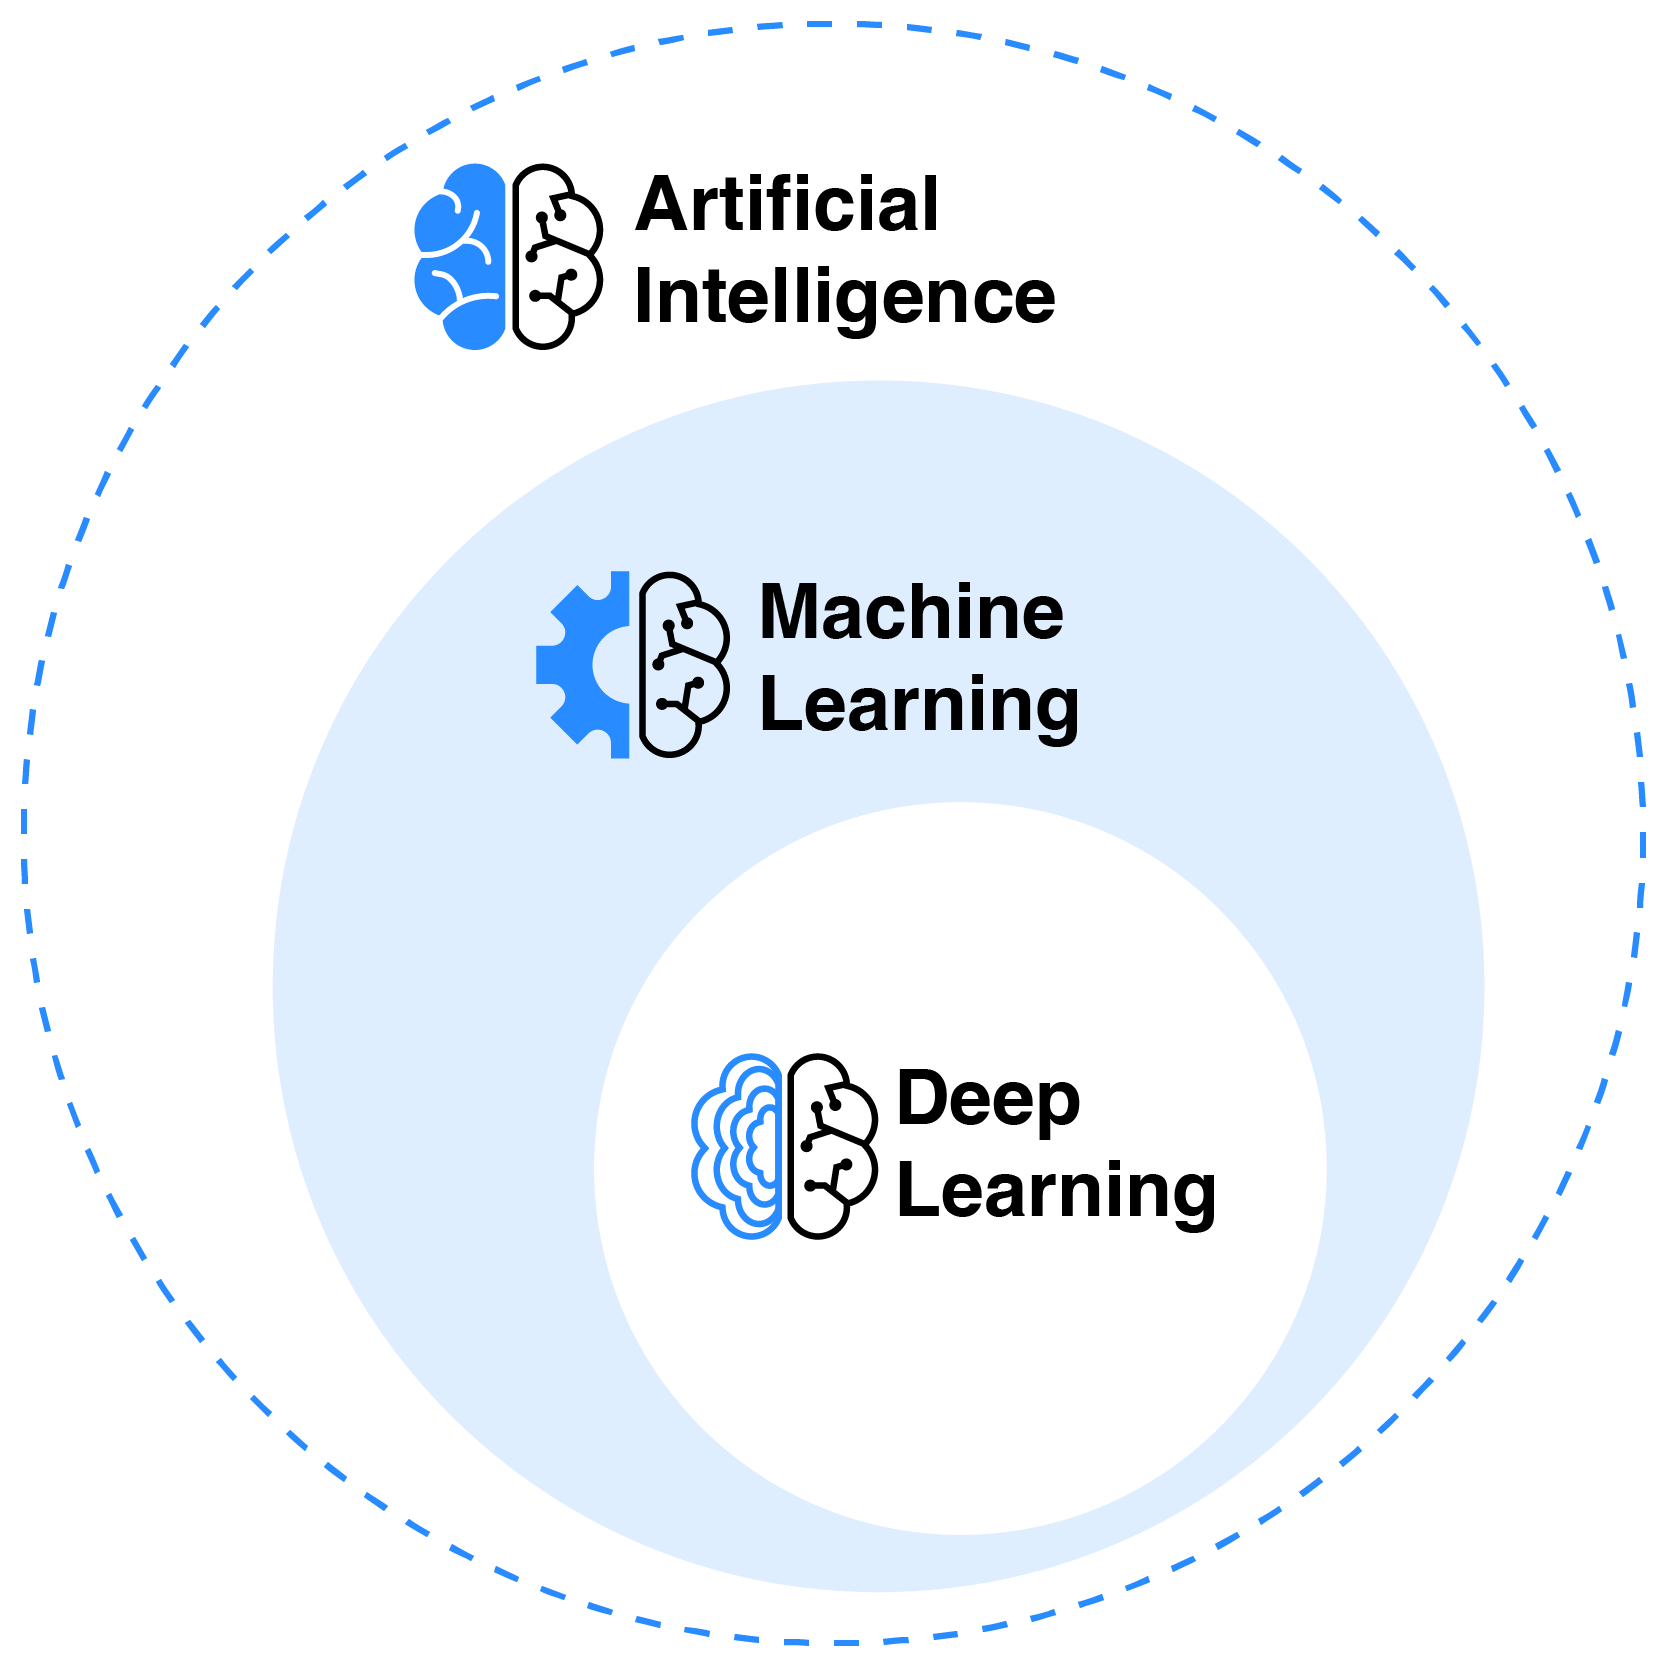
\includegraphics[width=0.5\linewidth]{reports//assets/ai.png}
    \caption[AI subsets overview]{Overview of AI subsets \cite{nasaWhatArtificialIntelligence}.}
    \label{fig:ai_overview}
\end{figure}


\subsection{Deep Learning in Medical Imaging}

The advent of DL techniques has profoundly transformed the field of medical imaging, enabling highly accurate analysis of complex visual data across a broad spectrum of clinical applications, including:

\begin{itemize}
    \item \textbf{Image classification and detection}: DL models are trained to identify and classify abnormalities in radiological images such as X-rays, MRI, or mammograms, often achieving expert-level performance.
    \item \textbf{Segmentation}: DL architectures facilitate the precise delineation of anatomical structures and pathological regions, which is essential for treatment planning, diagnosis, and disease monitoring.
    \item \textbf{Image enhancement and generation}: DL is employed to improve image quality (e.g., denoising, super-resolution) and to generate synthetic data for augmentation or cross-modality image synthesis.
\end{itemize}

These advancements have been largely driven by the success of Convolutional Neural Networks (CNNs), which have become the foundation of most state-of-the-art models in medical image analysis. CNN-based models are currently being actively explored for the classification of breast cancer molecular subtypes using mammography images, as recent studies have demonstrated their potential for this challenging task\cite{mota_breast_2024, ben_rabah_multimodal_2025}. For this reason, CNNs, particularly ResNet101, serve as the baseline architecture in this study. A detailed review of CNNs will be provided in the following section.



\section{Convolutional Neural Networks}

A Convolutional Neural Network (CNN) is a specialized type of DL model based on layers, designed to automatically learn and extract features from data, particularly images, by applying mathematical operations called convolutions. 

CNNs were first introduced by LeCun et al. \cite{lecun_gradient-based_1998} in their seminal work on LeNet (Figure \ref{fig:lenet}), an architecture developed for digit recognition. However, CNNs gained widespread popularity only after Krizhevsky et al. achieved a breakthrough in the 2012 ImageNet Large Scale Visual Recognition Challenge with their architecture, AlexNet \cite{NIPS2012_c399862d}.

The key innovation of CNNs lies in their ability to learn hierarchical features directly from raw data, reducing the need for manual feature engineering and enabling high performance across a variety of computer vision applications.


\begin{figure}[h!]
    \centering
    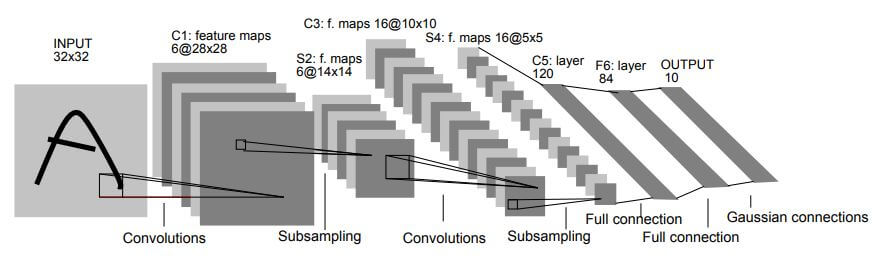
\includegraphics[width=0.8\linewidth]{reports//assets/lenet.jpg}
    \caption[LeNet CNN]{LeNet, considered the first CNN architecture for digit recognition \cite{lecun_gradient-based_1998}.}
    \label{fig:lenet}
\end{figure}


\subsection{Core Principles}

\textbf{Convolutional Layers}

A convolutional layer is the primary building block of a CNN. It applies a set of filters (or kernels) to the input data (image) by sliding each filter across the width and height while computing the dot product between the filter and the local region covered. This operation is known as convolution. The purpose of this operation is to generate a feature map, which highlights patterns or specific features of the input, like edges or textures \cite{noauthor_what_2021}. In a large CNN, this feature map is then propagated to the next layer to repeat the process and extract more complex features. Figure \ref{fig:convolution_feature_map} illustrates the convolution operation and a feature map example of a breast image.

\begin{figure}[h!]
	\centering
	\begin{subfigure}[c]{0.45\textwidth}
		\centering
		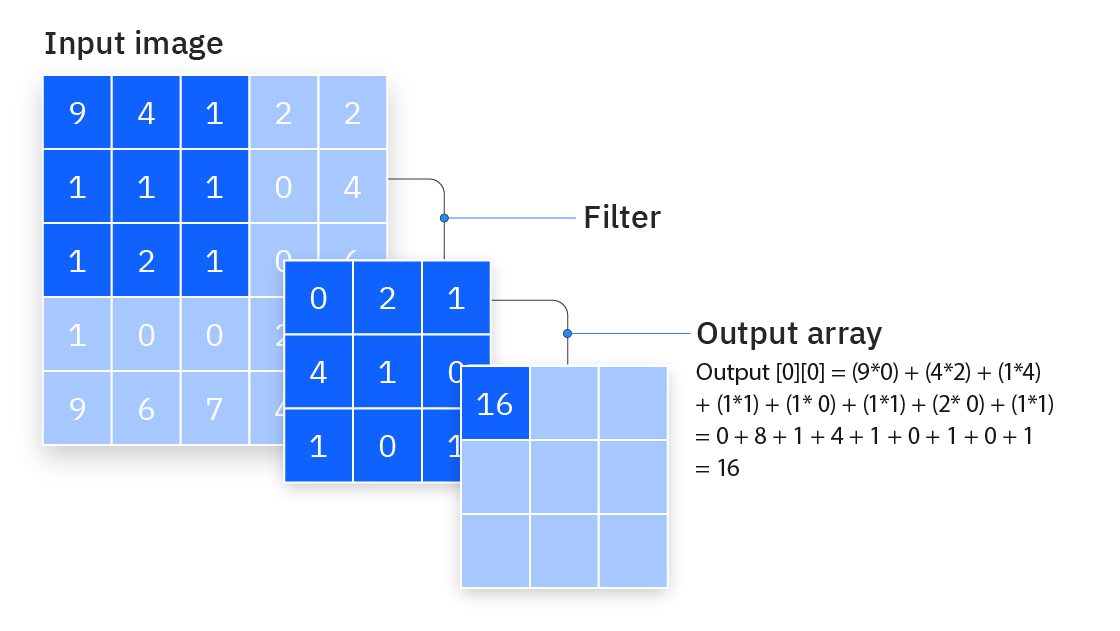
\includegraphics[width=\textwidth]{reports/assets/convolution.png}
            \caption{}
		\label{fig:convolution}
	\end{subfigure}
	\begin{subfigure}[c]{0.25\textwidth}
		\centering
		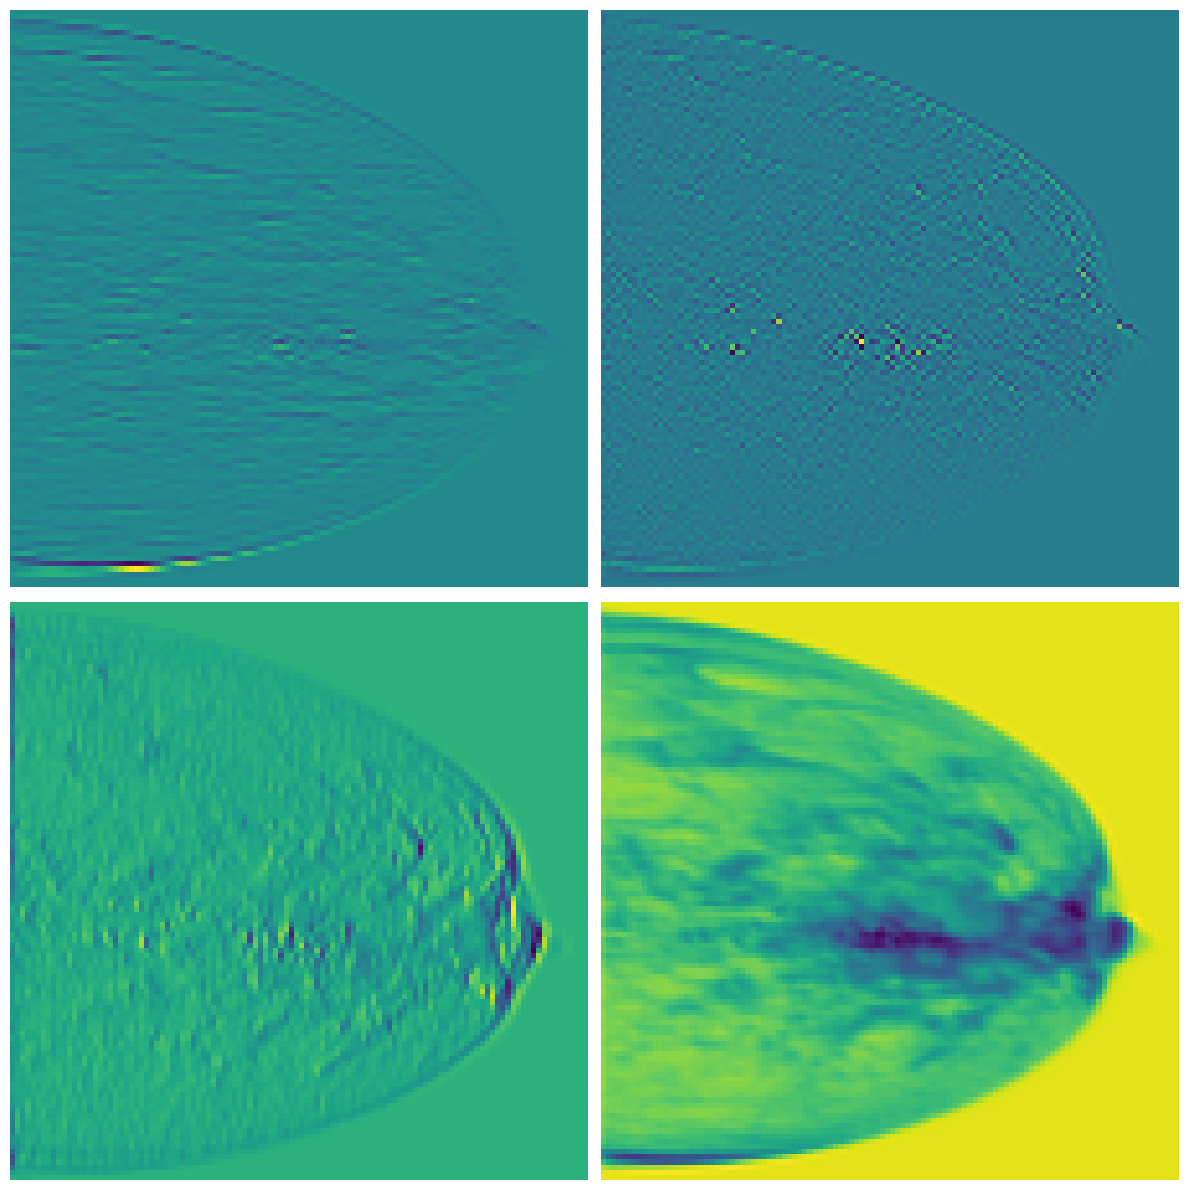
\includegraphics[width=\textwidth]{reports/assets/feature_maps_resnet.png}
            \caption{}
		\label{fig:feature_map_conv}
	\end{subfigure}
	\caption[Convolution and feature map]{(a) Illustration of the convolution operation \cite{noauthor_what_2021}. (b) Breast feature maps extracted from the first convolutional layer of Resnet101.}
\label{fig:convolution_feature_map}
\end{figure}

\textbf{Activation Functions}

Activation functions are mathematical functions used within neural networks. These functions are used to decide whether a neuron is activated or not, but most importantly, they introduce non-linearity into the network, enabling it to learn complex relationships beyond simple linear mappings. In simpler words, they help the network to understand more complex patterns, not just straight-line relationships \cite{langActivationFunctionsNeural2024}. Generally, activation functions are applied after the convolution operation to obtain the feature map. There are many activations functions, but the most used for CNN is the rectified linear unit (ReLU) due to its simplicity, computational efficiency and mitigation of the vanishing gradient problem \footnote{The difficulty of training deep learning networks due to gradients becoming very small as they propagate through many layers.}.

\begin{figure}
    \centering
    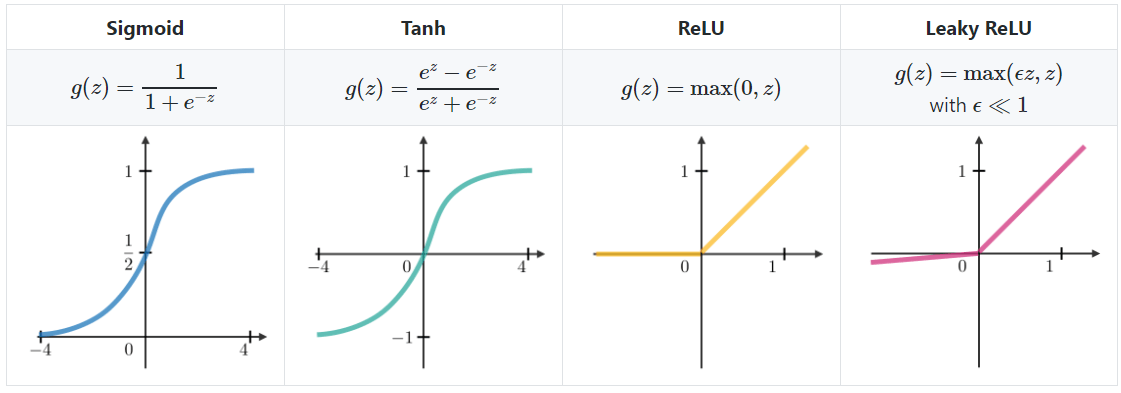
\includegraphics[width=1.0\linewidth]{reports//assets/activations_functions.png}
    \caption[Popular activation functions]{Popular activations functions used in CNN \cite{wachtelUnderstandingActivationFunctions2021}.}
    \label{fig:activations-functions}
\end{figure}

\textbf{Pooling Layers}

Pooling layers reduce the spatial dimensions of feature maps. This not only decreases computational complexity but also helps control overfitting\footnote{A common problem in machine learning where a model learns the training data too closely, rather than capturing patterns that generalize to new, unseen data.} \cite{brownlee_gentle_2019}. Unlike convolutional layers, pooling layers do not perform convolutions; instead, they apply a pooling operation to each region of the feature map. The two most popular pooling operations are max pooling, which selects the maximum value in each region and average pooling, which computes the mean value of the region (Figure \ref{fig:pooling_operations}). Pooling is typically applied after activation functions and is often repeated throughout the network. 

\begin{figure}[h!]
    \centering
    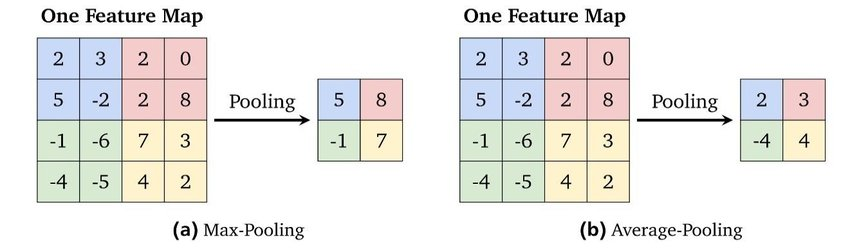
\includegraphics[width=1.0\linewidth]{reports//assets/pooling.png}
    \caption[Popular pooling operations]{Max pooling and Average pooling representation \cite{SkinLesionClassification}.}
    \label{fig:pooling_operations}
\end{figure}

\textbf{Fully Connected Layer}

Fully connected layers, also known as dense layers, are typically located near the end of a CNN. In these layers, every neuron is connected to every neuron in the previous layer, allowing the network to combine the features extracted by earlier convolutional and pooling layers into a global representation. Before entering the fully connected layers, the multidimensional feature maps are flattened into a one-dimensional vector, which serves as the input for these dense layers. This transformation enables the network to map the extracted features to the desired output, such as class probabilities \cite{noauthor_fully_nodate}. Figure \ref{fig:fc_layers} illustrates a neural network with several fully connected layers.

\begin{figure}[h!]
    \centering
    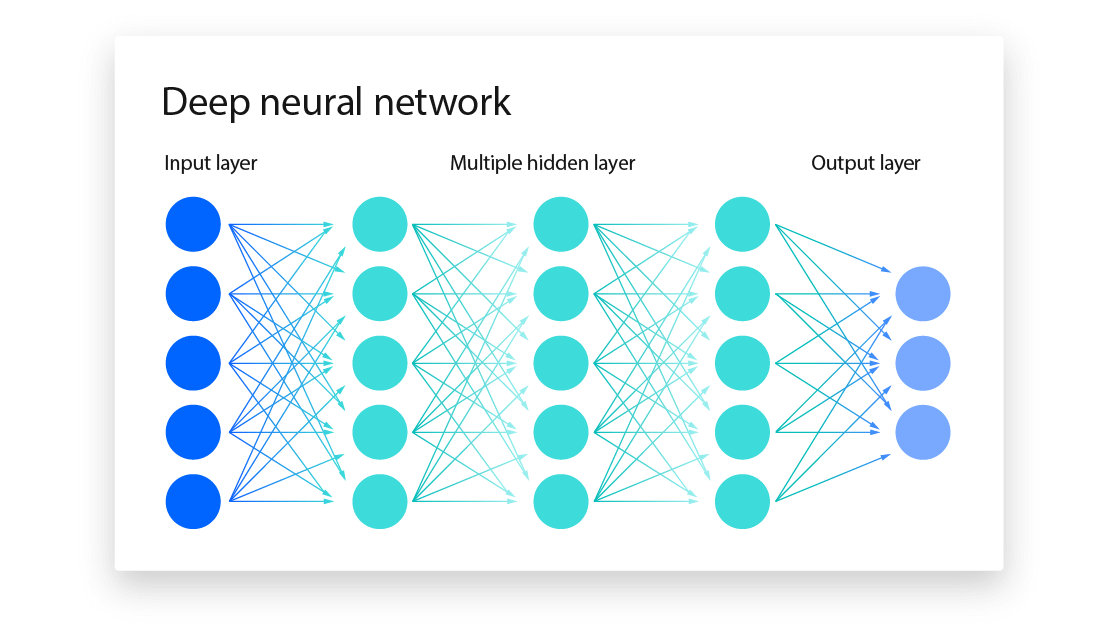
\includegraphics[width=0.75\linewidth]{reports//assets/fc_network.png}
    \caption[Fully connected layers]{Neural network with three fully connected layers and three outputs \cite{bergmann_what_2024}.}
    \label{fig:fc_layers}
\end{figure}

\textbf{Training}

With all this building blocks, CNN are constructed. Once a network is defined, it goes through the process of training, which involves the following steps \cite{bergmann_what_2024}:

\begin{enumerate}
    \item \textbf{Forward pass}: The input data passes through the network, layer by layer, to produce an output prediction.
    \item \textbf{Loss function calculation}: The difference between the predicted output and the true label is measured using a loss function.
    \item  \textbf{Backpropagation}: The network computes gradients of the loss with respect to each parameter, propagating the error backward through the layers.
    \item \textbf{Gradient descent}: The network updates its parameters (weights and biases) using the computed gradients to minimize the loss.
\end{enumerate}

After training, the network is ready to make predictions on new, unseen data. Figure \ref{fig:cnn_breast} shows an example of a complete CNN architecture for breast cancer prediction.

\begin{figure}[h!]
    \centering
    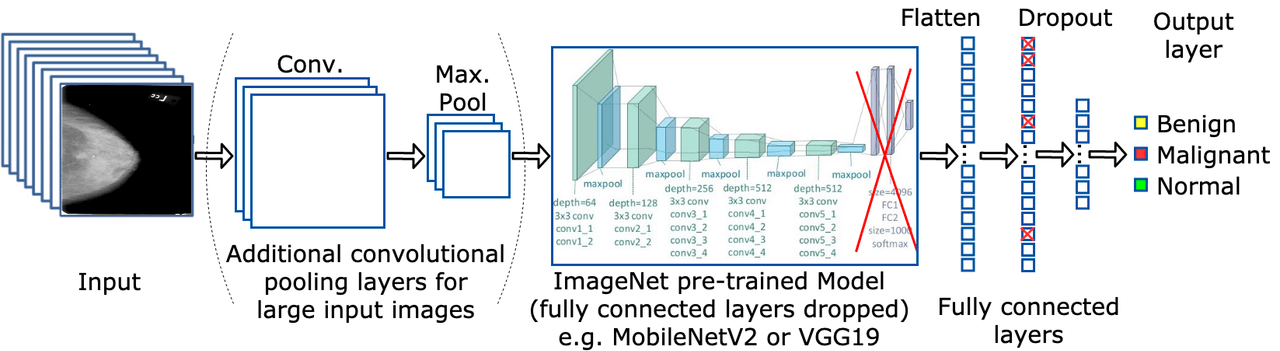
\includegraphics[width=0.75\linewidth]{reports//assets/cnn_breast.png}
    \caption[Breast cancer CNN]{CNN for breast cancer prediction \cite{jaamour_divide_2023}.}
    \label{fig:cnn_breast}
\end{figure}

\subsection{Main Architectures}

\textbf{VGGNet (VGG16/VGG19)}

Symonyan et al. (2015) introduced VGGNets \cite{simonyanVeryDeepConvolutional}. Renowned for their straightforward design and depth, they employ solely 3×3 convolutions and can have up to 19 layers. They are extensively utilized as feature extractors and serve as a fundamental benchmark for transfer learning in both medical and general image applications.

\textbf{ResNet}

He et al. (2015) \cite{he_deep_2015} presented Residual Networks, or ResNets, as a solution for training very deep neural networks with over 50 layers, which helps address the problem of vanishing gradients. This is achieved through the implementation of residual or skip connections between layers. ResNet is the default choice for many image analysis tasks due to its robustness and ease of training.

\textbf{MobileNet}

As introduced by Howard et al. (2017) \cite{howardMobileNetsEfficientConvolutional2017}, MobileNet was specifically engineered for mobile and embedded systems. By utilizing depthwise separable convolutions\footnote{A different kind of convolution that splits the process in two steps: filtering each input channel and then combining them with a 1×1 convolution.}, it effectively decreases computational requirements and model size, rendering it highly suitable for real-time and resource-limited applications.

As previously stated, this study uses ResNet-101 as the baseline model. This architecture, comprised of 101 layers with residual connections, proves highly performance at managing complex tasks. Figure \ref{fig:resnet_101} illustrate an overview of its structure.

\begin{figure}[h!]
    \centering
    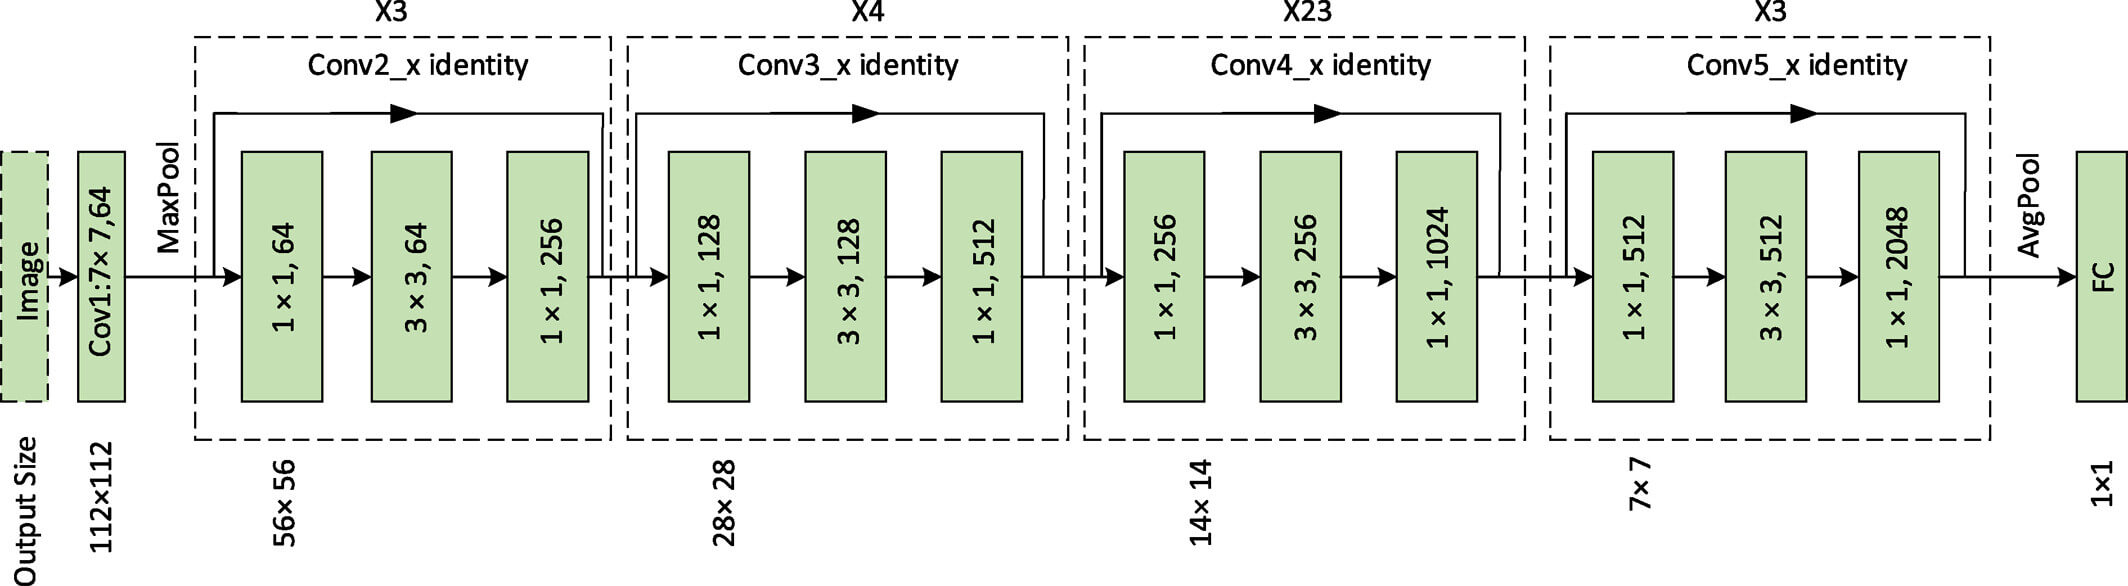
\includegraphics[width=0.75\linewidth]{reports//assets/resnet101.jpg}
    \caption[ResNet-101 Architecture]{ResNet-101 Architecture.}
    \label{fig:resnet_101}
\end{figure}


\subsection{CNNs Limitations}

CNNs offer numerous advantages and a wide range of applications; however, they also have certain limitations that deserve consideration:

\begin{itemize}
    \item \textbf{Limited global context}: CNNs primarily focus on local features within small receptive fields, which limits their ability to capture long-range dependencies or global spatial relationships across an image. This can be a drawback in medical imaging, where understanding the broader anatomical context is often crucial.
    
    \item \textbf{Rigid inductive bias}: The architectural design of CNNs imposes strong assumptions of locality and translation invariance. While this is effective for many visual tasks, it can restrict the model’s flexibility to learn more abstract or non-local patterns that may be relevant in heterogeneous medical images.
    
    \item \textbf{Generalization across diverse data}: CNNs often struggle to generalize when applied to data from different hospitals, imaging devices, or patient populations, due to domain shifts and variability in medical imaging protocols. This lack of robustness can hinder their reliability in real-world clinical practice.
\end{itemize}

Recent advances in Transformer-based models offer promising solutions to some of these limitations by enabling better modeling of global context and improving generalization, which will be discussed in the following section.

\section{Transformer-Based models}

Transformer models are built upon the Transformer architecture, which was initially developed for natural language processing (NLP) tasks. Since their introduction to computer vision, these models have gained significant popularity as an alternative to CNNs due to their effectiveness in capturing global context and modeling long-range dependencies within images \cite{pereira_review_2024}. 

In this section, we review what transformer-based models are and describe the architectural designs of those analyzed in this work for the task of breast cancer molecular subtype classification.

\subsection{The Transformer architecture}

The Transformer architecture is a DL model introduced by Vaswani et al. (2017) in their seminal paper “Attention is All You Need” \cite{vaswani_attention_2017}. Originally developed as an alternative to recurrent neural networks (RNNs)\footnote{A special class of artificial neural network designed to process sequential or time-series data, such as text, speech, or sensor readings.} for sequence-to-sequence tasks in NLP, the Transformer has since become widely adopted in computer vision as well.

At its core, the Transformer consists of an encoder-decoder structure built from repeated layers containing two key components: multi-head self-attention and position-wise feed-forward networks (see Figure~\ref{fig:transformer}). This design enables the model to capture both local and global dependencies by relating every element in the input sequence to every other element, regardless of their positions.

\begin{figure}[h!]
    \centering
    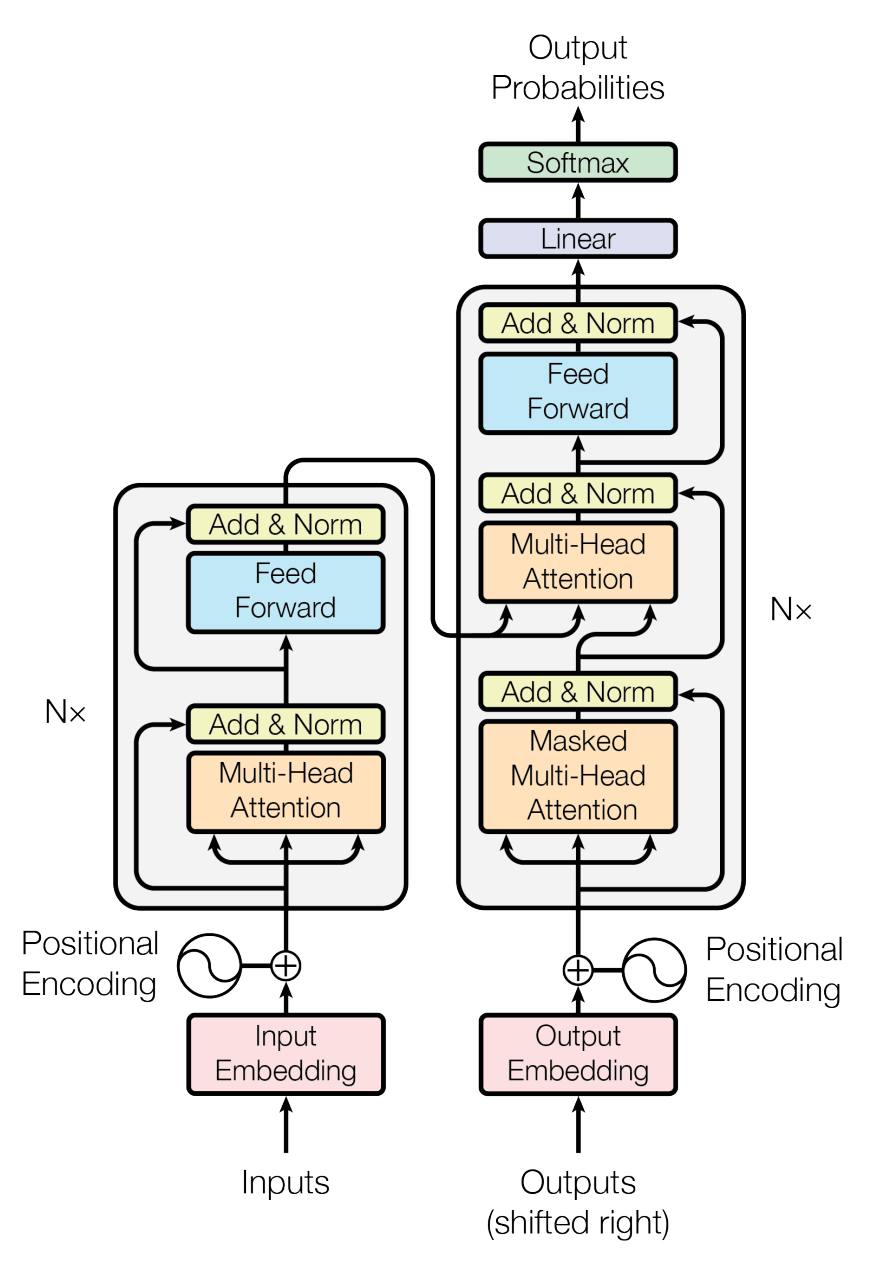
\includegraphics[width=0.5\linewidth]{reports//assets/transformer.png}
    \caption[Transformer Architecture]{The Transformer Architecture \cite{vaswani_attention_2017}.}
    \label{fig:transformer}
\end{figure}

\textbf{Self-Attention}

Self-attention is an attention mechanism\footnote{A technique in machine learning that enables models to focus on the most relevant parts of the input data when making predictions or generating outputs.} that allows a network to relate different positions within a single input sequence, thereby computing a context-aware representation for each element. In simpler terms, it enables the model to efficiently prioritize and integrate important information from across the entire input. The concept of attention was first introduced by Bahdanau et al. (2014) \cite{bahdanau_neural_2014}, but it was the Transformer architecture that first relied entirely on self-attention to compute representations \cite{vaswani_attention_2017}. In a concise overview, this process functions as follows:

\begin{itemize}
    \item \textbf{Projection}: Each input element is projected into three distinct vectors:
        \begin{itemize}
        \item \textbf{Query (Q)}: Represents the current element (e.g., a word or image patch) for which we want to find relevant information from the sequence.
        \item \textbf{Key (K)}: Represents each element in the sequence and is used to match against queries to measure their relevance.
        \item \textbf{Value (V)}: Contains the actual information of each element, which will be combined according to the attention scores.
        \end{itemize}
    \item \textbf{Score Calculation}: For each element, an attention score is computed by taking the dot product between its query and all keys in the sequence.
    \item \textbf{Scaling}: Each score is divided by the square root of the key dimension to stabilize training and prevent large gradients.
    \item \textbf{Softmax Normalization}: The softmax\footnote{The softmax function transforms the scores into probabilities that sum to one.} function is applied to the scaled scores to obtain attention weights.
    \item \textbf{Weighted Sum}: A new, context-aware representation for each input element is obtained by computing the weighted sum of all value vectors using the attention weights.
\end{itemize}

Figure \ref{fig:scaled_dot_product_attn} illustrates the process of scaled dot-product attention in detail. Mathematically, the process can be summarized as follows:

$$Attention(Q,K,V) = softmax\left(\frac{QK^T}{\sqrt{d_k}}\right)V$$

\begin{figure}[h!]
    \centering
    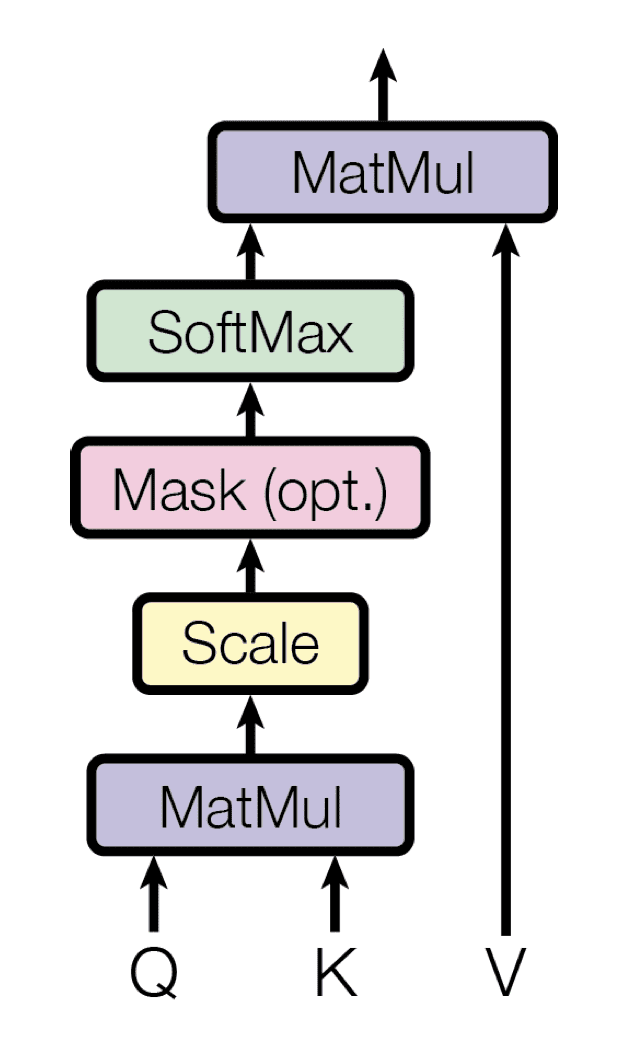
\includegraphics[width=0.3\linewidth]{reports//assets/scaled_dot_product.png}
    \caption[Scaled dot-product attention]{Scaled dot-product attention mechanism \cite{vaswani_attention_2017}.}
    \label{fig:scaled_dot_product_attn}
\end{figure}


\subsection{Vision Transformer}

A Vision Transformer (ViT) is a DL  architecture introduce by Dosovitskiy et al. (2020) \cite{dosovitskiy_image_2020} designed for computer vision tasks, inspired by the Transformer architecture originally developed for NLP. 

\textbf{ViT processing pipeline}

A ViT processes an image by first dividing it into fixed-size patches, for example, a 224×224 image split into 16×16 patches results in 196 patches. Each patch is then flattened and projected into an embedding space by the patch embedding layer. Because the ViT architecture lacks inherent spatial awareness, positional encodings are added to each patch embedding to preserve spatial information within the image. This design allows the input to be treated analogously to a sequence of tokens in NLP Transformers. As the sequence passes through multiple layers of multi-head self-attention, the model learns to capture both local and global relationships among the patches, enabling robust image understanding. This process and the ViT architecture is depicted in the Figure \ref{fig:vit_arch}.


\begin{figure}[h!]
    \centering
    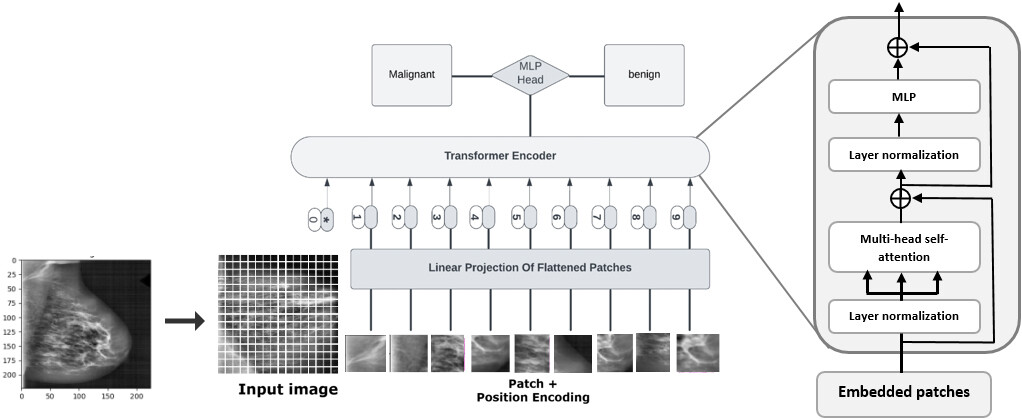
\includegraphics[width=1.0\linewidth]{reports//assets/vit_breast.jpg}
    \caption[Vision Transformer Architecture]{ViT architecture, in this example, for breast cancer classification \cite{abimouloud_vision_2024}.}
    \label{fig:vit_arch}
\end{figure}

ViTs have rapidly expanded their reach to many computer vision tasks, including image classification, object detection, and image segmentation. In medical imaging, several studies have evaluated their performance on tasks such as breast cancer classification, consistently reporting strong results \cite{marquez_vara_vision_2024, mauricio_comparing_2023, ayana_vision-transformer-based_2023}.


\subsection{Shifted-Window Transformer}

Shifted-Window Transformers (Swin), introduced by Liu et al. (2021) \cite{liu_swin_2021}, are a specialized architecture derived from Vision Transformers (ViT). They are designed to address some of the limitations of ViT, particularly regarding computational efficiency and scalability when processing high-resolution images.

To achieve this, Swin employs a shifted window mechanism. Unlike ViT, which typically applies self-attention globally, Swin divides the image into a set of non-overlapping windows (Figure \ref{fig:swin_vit}), with each window containing a subset of image patches. Self-attention is then applied locally within each window, significantly reducing computational complexity. The windows are shifted between layers to enable cross-window connections and enhance information flow across the entire image.

\begin{figure}[h!]
    \centering
    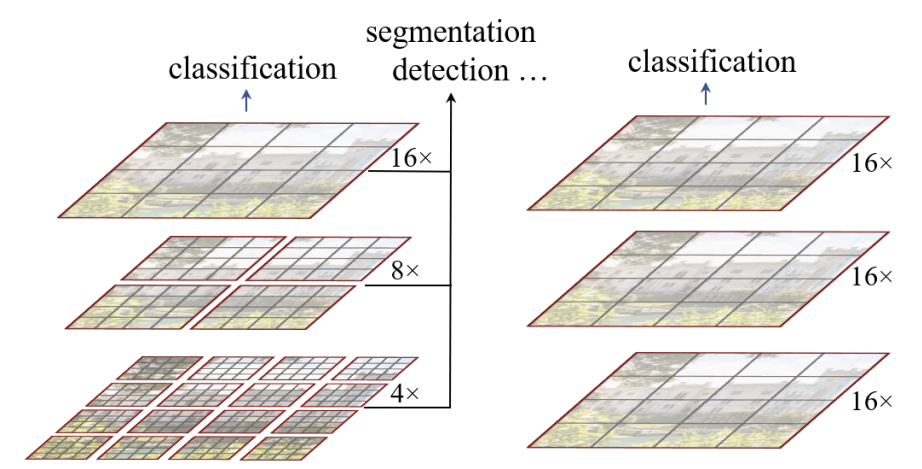
\includegraphics[width=0.6\linewidth]{reports//assets/Swin.png}
    \caption[Comparison of Swin and ViT mechanisms]{Comparison of Swin and ViT attention mechanisms. \textbf{Left:} Swin Transformer with shifted window self-attention. \textbf{Right:} Vision Transformer (ViT) with global self-attention across all patches \cite{liu_swin_2021}.}
    \label{fig:swin_vit}
\end{figure}

As a result of this mechanism, Swin exhibits a computational complexity of $O(n)$, whereas ViT has a complexity of $O(N^2)$. 



\begin{figure}[h!]
    \centering
    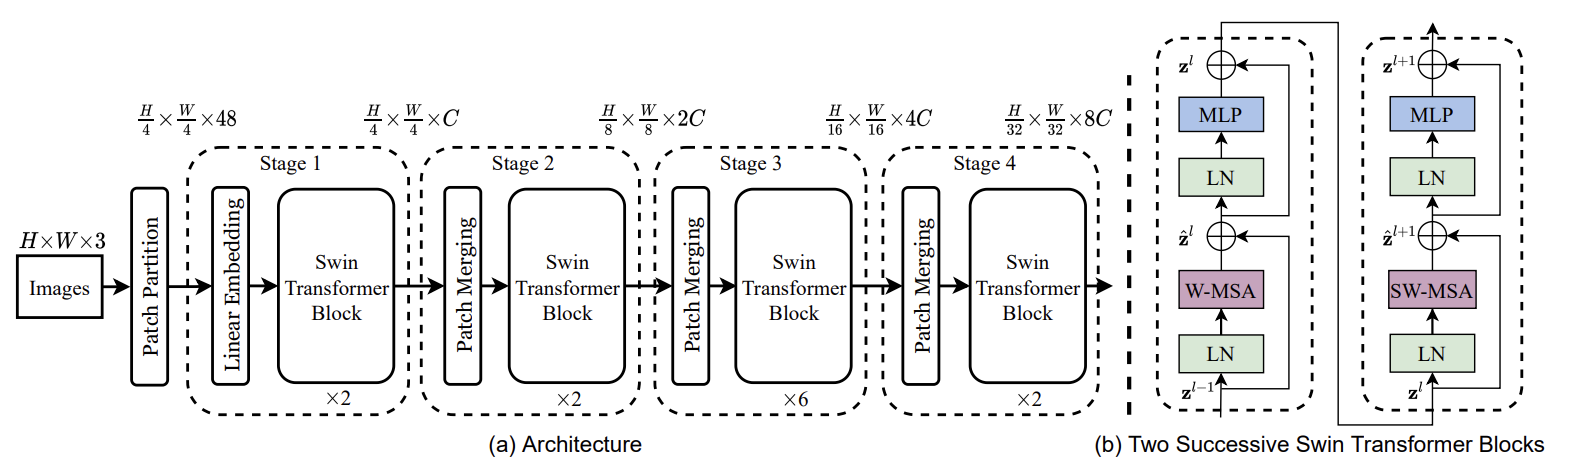
\includegraphics[width=1.0\linewidth]{reports//assets/SwinArch.png}
    \caption[Swin Transformer Arch]{Swin Transformer Architecture \cite{liu_swin_2021}.}
    \label{fig:swin_arch}
\end{figure}

\subsection{Multi-Axis Vision Transformer}

Multi-Axis Vision Transformer (MaxViT) is a hybrid vision transformer architecture introduced by Tu et al. (2022) \cite{tu_maxvit_2022}. It is designed to capture both local and global spatial relationships in images, overcoming scalability and capacity limitations of previous transformer-based models. MaxViT achieves this by combining blocked local attention (as in Swin, but without shifting) and dilated global (grid) attention within each block, together with convolutional layers. This multi-axis attention mechanism allows MaxViT to efficiently model both short- and long-range dependencies while maintaining the same linear computational complexity as Swin. Figure \ref{fig:max_vit_arch} illustrates this structure.

\begin{figure}[h!]
    \centering
    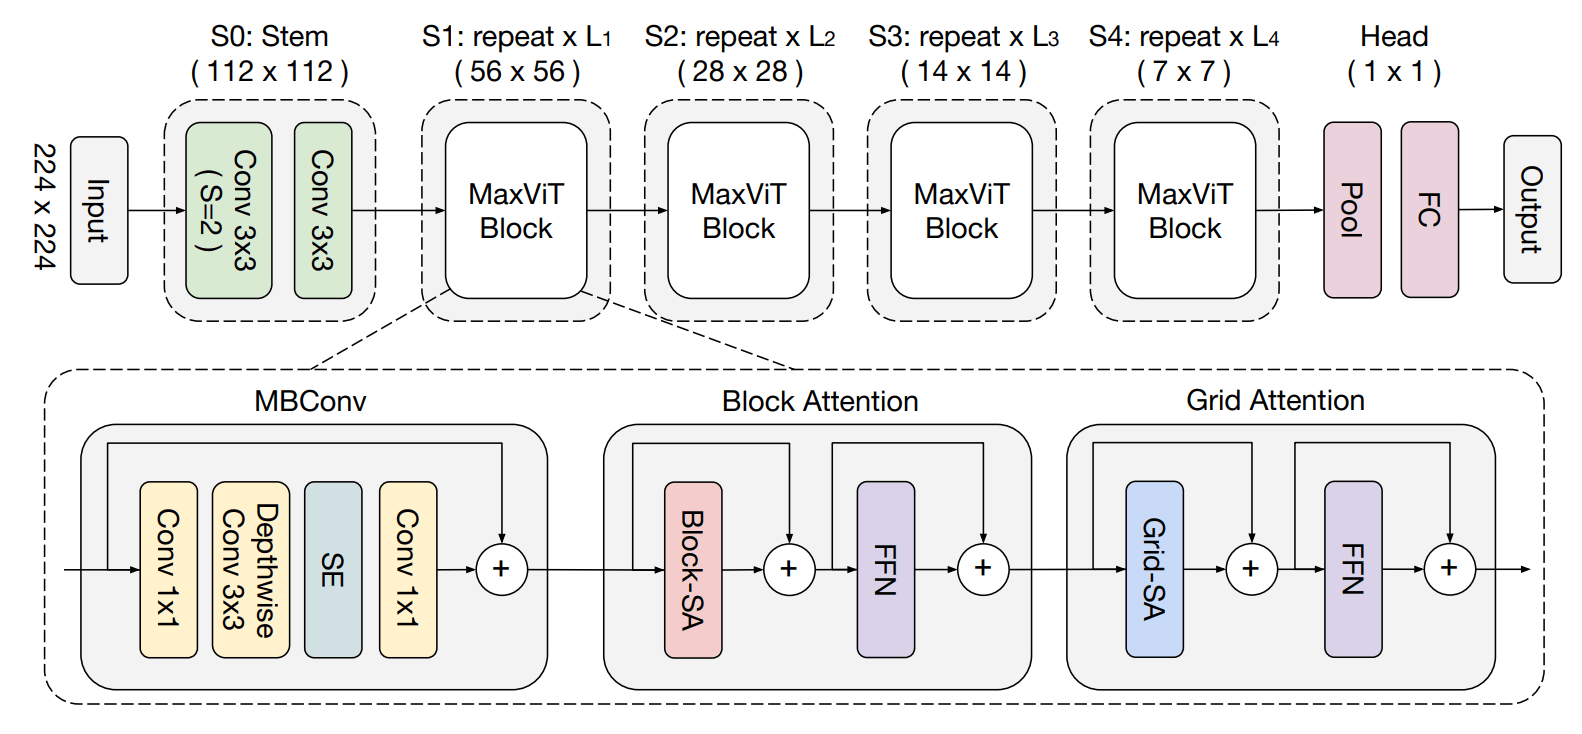
\includegraphics[width=1.0\linewidth]{reports//assets/maxvit_arch.png}
    \caption[Multi-Axis Vision Transformer Arch]{MaxVit Architecture \cite{tu_maxvit_2022}.}
    \label{fig:max_vit_arch}
\end{figure}


\textbf{Multi-Axis Attention}

Multi-axis attention is the key component of MaxViT. It works by splitting the attention mechanism into two parts: a block of local attention, which focuses on local regions (similar to Swin’s), and a grid attention block, which enables global information flow across the entire image through a dilated, grid-like pattern. This design allows MaxViT to efficiently capture both local and global dependencies within each block (see Figure \ref{fig:multi_axis_attention}).

\begin{figure}[h!]
    \centering
    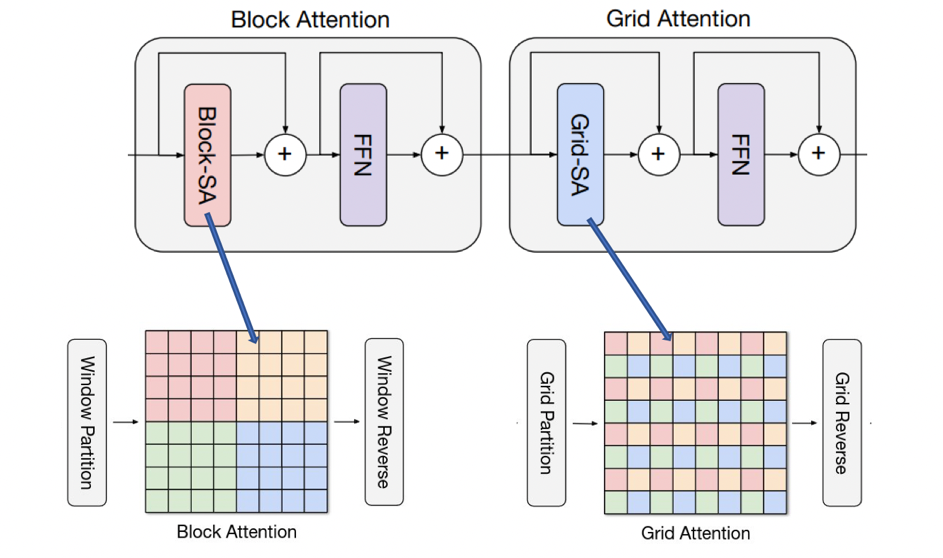
\includegraphics[width=0.6\linewidth]{reports//assets/multi_axis_attention.png}
    \caption[Multi-Axis Attention Blocks]{Multi-Axis attention blocks \cite{noauthor_maxvit-unet_2024}.}
    \label{fig:multi_axis_attention}
\end{figure}


\section{Training and Evaluation Techniques}
\subsection{Transfer Learning}

Transfer learning is a ML technique in which a model developed and trained on one task or dataset is reused or fine-tuned to improve performance on a different, but related, task. It is especially valuable when data is limited or the target task has few labeled examples available \cite{murel_what_2024}. In other words, instead of training a new model from scratch, transfer learning leverages knowledge previously obtained—such as learned features and weights, often from large datasets—to accelerate and enhance learning on a new problem.

This approach is very popular and widely used to avoid training new machine learning or deep learning models from scratch. In medical imaging, for example, where annotated data is often scarce or expensive to obtain, transfer learning has enabled the development and training of models that reduce training time, improve performance, and promote feature reuse \cite{matsoukas_what_2022}. This process is depicted in Figure \ref{fig:transfer_learning}.

\begin{figure}[h!]
    \centering
    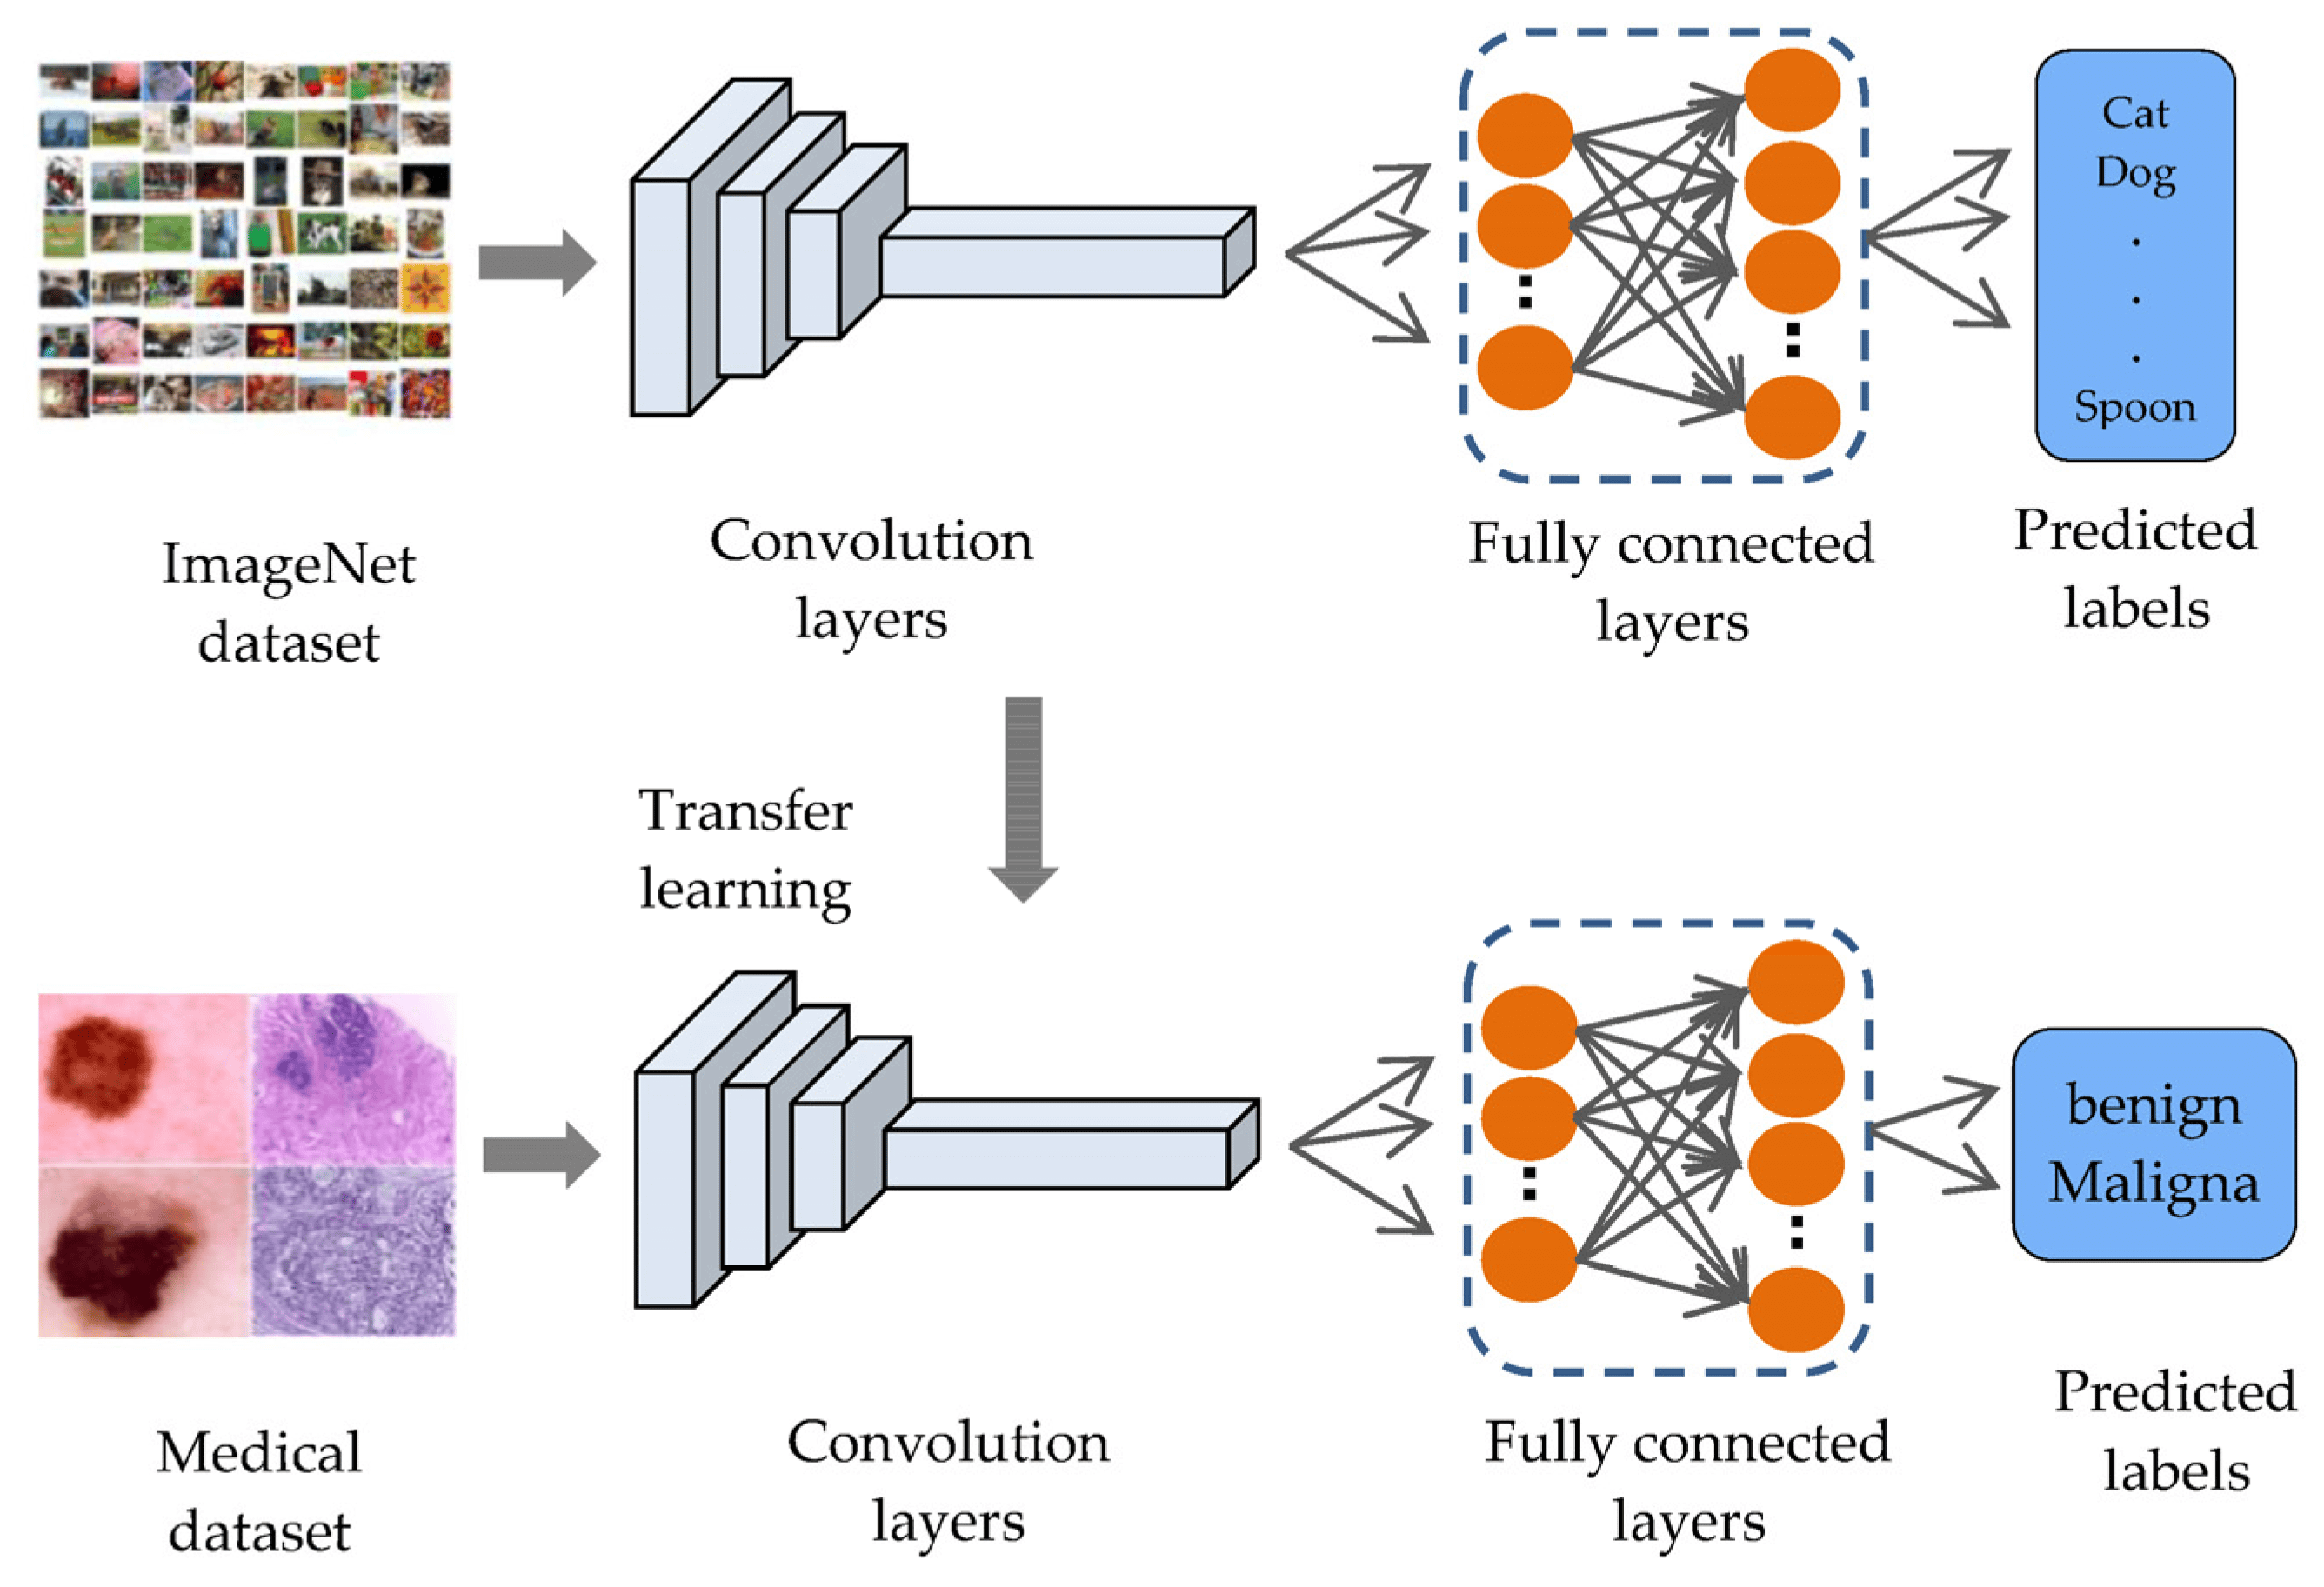
\includegraphics[width=0.75\linewidth]{reports//assets/transfer-learning.png}
    \caption[Transfer learning process]{Transfer learning process where}
    \label{fig:transfer_learning}
\end{figure}


\subsection{Fine-Tuning}

Fine-tuning is a specific technique within transfer learning that involves taking a pre-trained model and continuing its training on a smaller or more specialized dataset to adapt its capabilities to a particular case or domain \cite{noauthor_what_2024}. During fine-tuning, some or all of the model’s parameters are unfrozen and updated, allowing the model to learn features relevant to the new task while retaining the general knowledge acquired during pre-training. However, training large models on small datasets can lead to overfitting, so it is common practice to use a lower learning rate during fine-tuning to make gradual adjustments and preserve previously learned representations.

\subsection{K-Fold Cross-Validation}

When training ML or DL models, it is standard practice to split the dataset into separate subsets, typically train, validation, or test sets. The training set is used to fit the model, while the test set serves to evaluate its performance on unseen data. This approach helps estimate how well the model will generalize to new data and prevents overfitting by ensuring that evaluation is performed on data not used during training.

However, when data is limited or there are concerns about the reliability of a single train/test split, a more robust evaluation method is required. In these cases, K-Fold Cross-Validation is commonly used.

K-Fold Cross-Validation works by dividing the dataset into $K$ equally sized folds. The model is trained and validated $K$ times, each time using a different fold as the validation set and the remaining folds for training. This ensures that every data point, image, or sample is used for both training and validation, providing a less biased and more reliable estimate of model performance compared to a simple train/test split. By averaging the results across all folds, K-Fold Cross-Validation reduces the variance associated with a single split and offers a comprehensive assessment, especially valuable when working with small or imbalanced datasets. Figure \ref{fig:k_fold} illustrates this process.

\begin{figure}[h!]
    \centering
    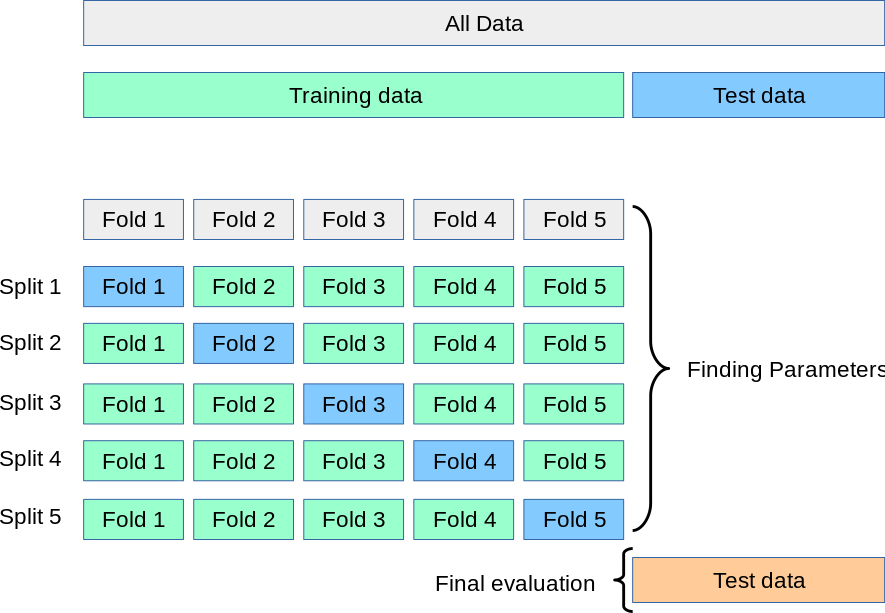
\includegraphics[width=0.75\linewidth]{reports//assets/k-fold.png}
    \caption[K-Fold Cross Validation]{K-Fold cross validation process, in this example, $K$ = 5 \cite{noauthor_31_nodate}.}
    \label{fig:k_fold}
\end{figure}

\subsection{AI Explainability}

\textbf{Grad-CAM}

\textbf{Attention-Rollout}

\chapter{Materials and Methods}

This section documents the materials and processes carried out for this study. First, the selected dataset for model training and analysis is described, followed by the processing and preparation of the images, and finally the evaluation metrics used to assess model performance.

\section{The Chinese Mammography Database}

The Chinese Mammography Database (CMMD) is a public dataset developed by Cai et al. (2023) \cite{cai_online_2023} and hosted on The Cancer Imaging Archive (TCIA)\footnote{\url{https://www.cancerimagingarchive.net/collection/cmmd/}}. This dataset includes a total of 3,712 mammograms from 1,775 Chinese patients, in craniocaudal (CC) and mediolateral oblique (MLO) views, collected between July 2012 and January 2016. CMMD is divided into two subsets: CMMD1, which contains studies with basic clinical information, and CMMD2, which also includes molecular subtype annotations. The latter is the main basis for this research, as it is the only public and freely accessible subset that provides such molecular labels explicitly. Table \ref{tab:cmmd_features} details the main characteristics of each subset.

\begin{table}
        \caption[CMMD subsets characteristics]{Main characteristics of the CMMD subsets}
	\centering
	\begin{tabular}{lccccc}
		\toprule
		                            & \textbf{CMMD1}       & \textbf{CMMD2}      &      \\
		\midrule
		\textbf{Number of patients} & 1026                 & 749                 & 1775 \\
		\textbf{Number of images}   & 2214                 & 1498                & 3712 \\
		\textbf{Mean patient age}   & 45.92 (17-84 years)  & 49.82 (21-87 years) & -    \\
		\textbf{Categories}         & Benign and Malignant & Malignant only      & -    \\
		\textbf{Molecular subtype}  & No                   & Yes                 & -    \\
		\bottomrule
	\end{tabular}
	\label{tab:cmmd_features}
\end{table}


\subsection{General Description}

As mentioned above, the focus of this study is on the CMMD2 subset. For its composition, only malignant cases with complete immunohistochemical marker information and a diagnosis of invasive carcinoma were selected, as detailed in the exclusion criteria shown in Figure \ref{fig:cmmd_criteria}. After applying these criteria, the final sample consisted of 1,498 images corresponding to 749 patients.

\begin{figure}[h]
	\centering
	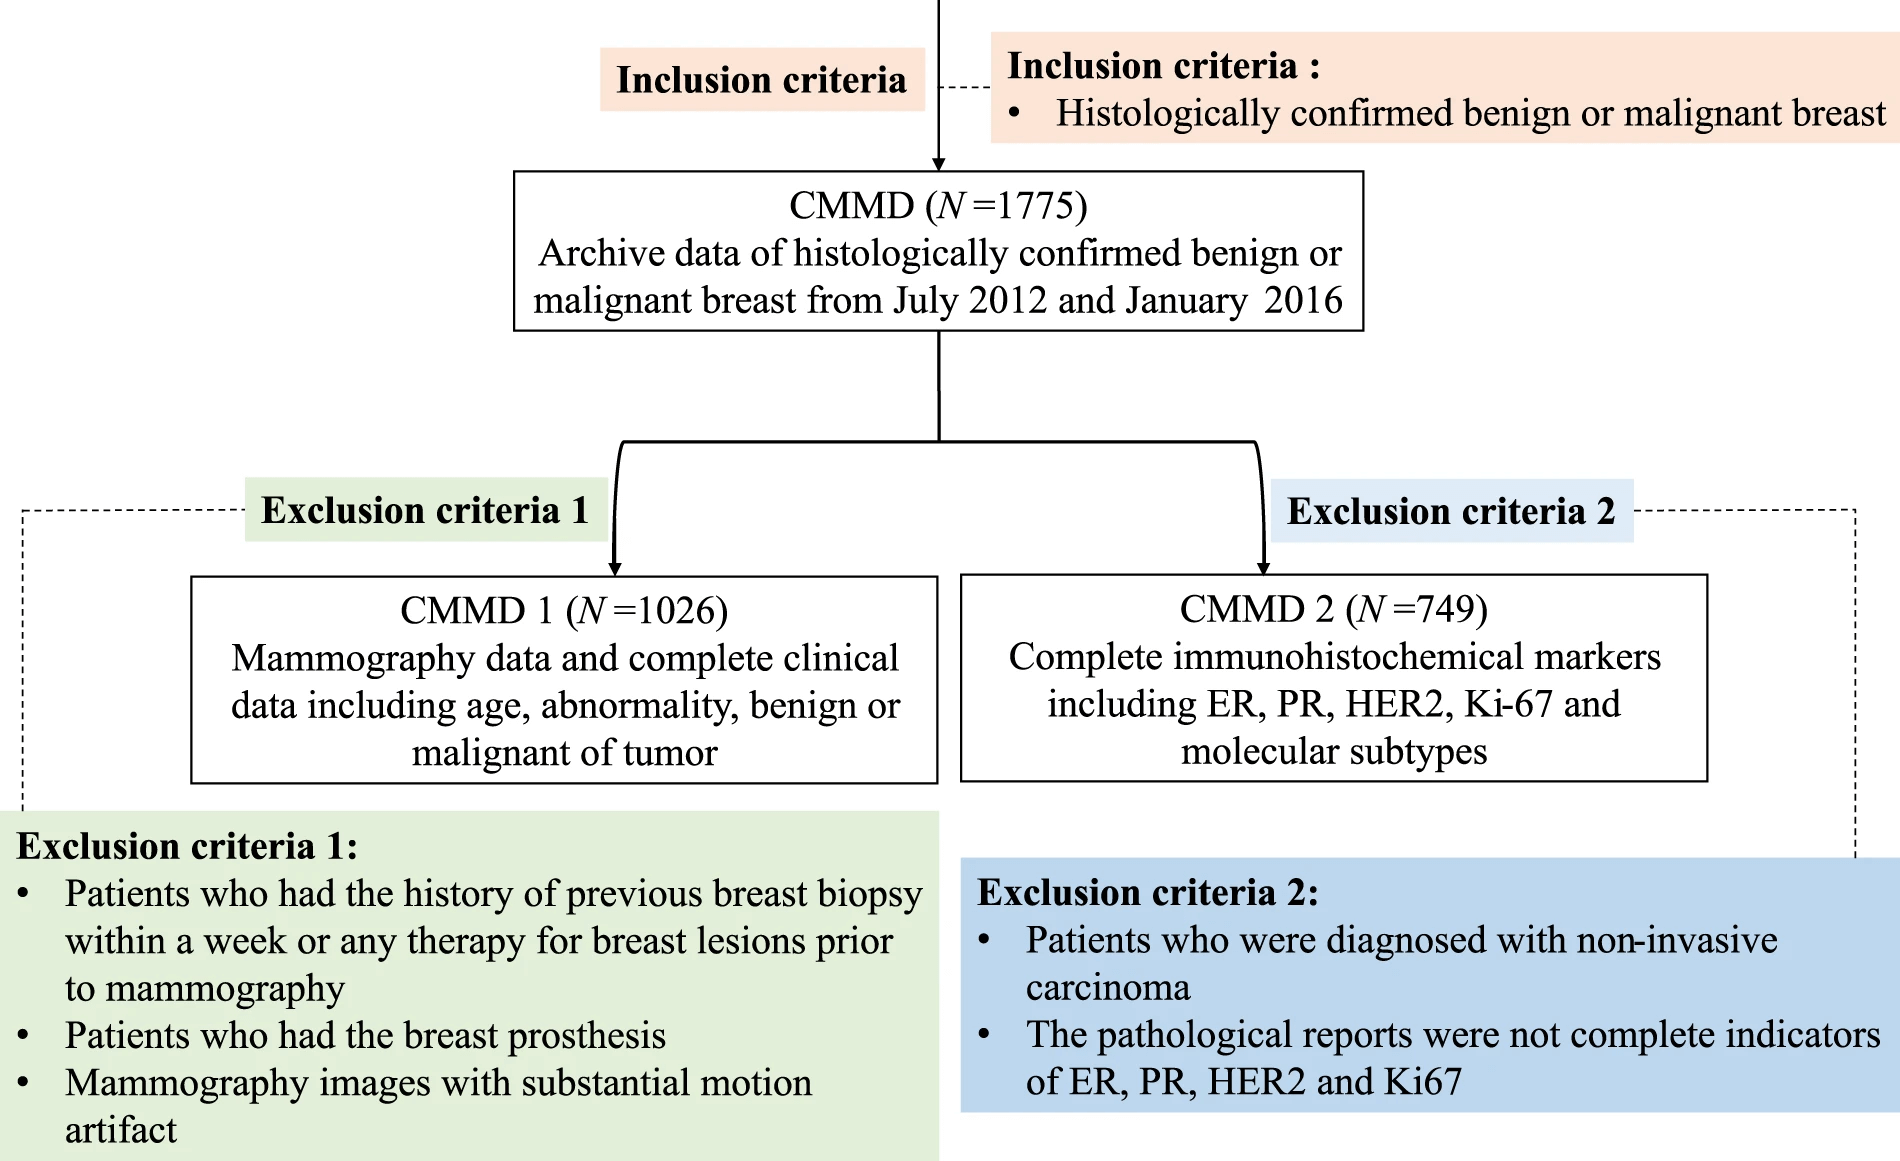
\includegraphics[width=0.8\linewidth]{reports//assets/cmmd_criteria.png}
	\caption[CMMD's inclusion and exclusion criteria]{CMMD's inclusion and exclusion criteria \cite{cai_online_2023}.}
	\label{fig:cmmd_criteria}
\end{figure}

\textbf{Image Collection}

The mammography images were collected using the \textbf{GE Senographe DS} mammography system, obtaining both CC and MLO views for each patient. The images were then stored in 8-bit grayscale at a image size of 2294×1914 pixels \cite{cai_online_2023}.

\textbf{Image Format and Resolution}

The main format of the images in the dataset is DICOM (Digital Imaging and Communications in Medicine), the standard in medical imaging, as it allows clinical metadata to be stored alongside the image and enables interoperability between equipment from different manufacturers as well as interaction between different information systems in hospitals and healthcare centers.

\newpage
\subsection{Metadata}

For each patient, the dataset provides a CSV\footnote{A plain text file that stores data in tabular form, where each line represents a row and each value in the row is separated by a comma} (Comma Separated Values) file with additional information to the obtained images, including age, laterality, type of abnormality, classification, and in the case of CMMD2, also the molecular subtype of the tumor. Table \ref{tab:cmmd2_metadata} describes these data in detail.

\begin{table}[h]
	\caption[CMMD2 metadata description]{Description of metadata variables present in the CMMD dataset.}
	\centering
	\begin{tabular}{>{\bfseries}l p{5cm} p{6cm}}
		\toprule
		\textbf{Column} & \textbf{Description}                 & \textbf{Possible values}                             \\
		\midrule
		ID1             & Unique patient identifier            & Format: D2-XXXX                                      \\
		LeftRight       & Breast laterality                    & L (left), R (right)                                  \\
		Age             & Patient age at the time of the study & Between 21 and 87 years                              \\
		Number          & Number of images available per study & Between 2 and 4                                      \\
		Abnormality     & Type of abnormality                  & Mass, Calcification, Both                            \\
		Classification  & Nature of the abnormality            & Benign, Malignant                                    \\
		Subtype         & Molecular subtype of breast cancer   & Luminal A, Luminal B, HER2-enriched, Triple negative \\
		\bottomrule
	\end{tabular}

	\label{tab:cmmd2_metadata}
\end{table}

It is important to note that, in the case of CMMD2, the laterality column indicates the side where the tumor was found; therefore, the opposite side is considered benign \cite{cai_online_2023}.

The age distribution of patients follows an approximately normal distribution with slight asymmetries. The most frequent age range is between 45 and 55 years, which is consistent with breast cancer epidemiology, where the majority of cases are diagnosed during this age interval [citation needed]. The inclusion of younger patients in the dataset enhances population diversity and enables analysis of model performance across underrepresented demographic subgroups.

\begin{figure}[h!]
	\centering
	\begin{subfigure}[c]{0.49\textwidth}
		\centering
		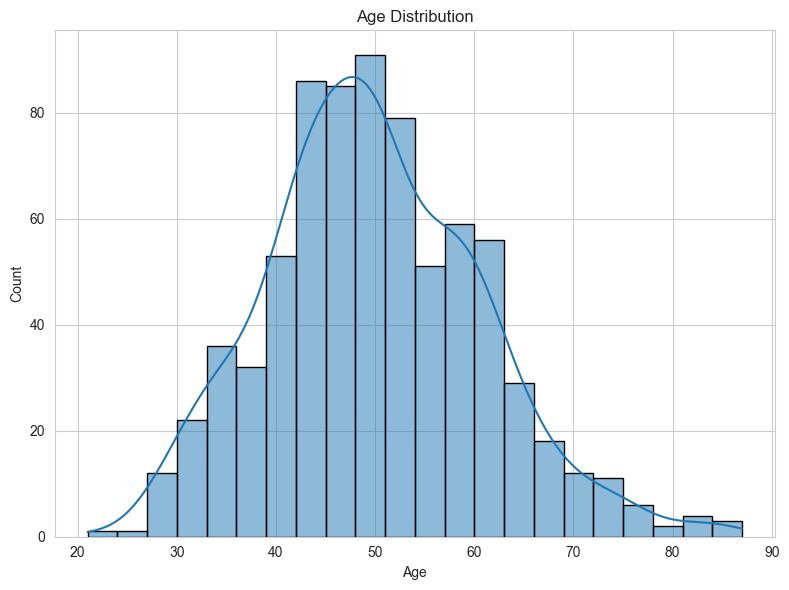
\includegraphics[width=\textwidth]{reports//assets/age.png}
		\caption{Age distribution}
		\label{fig:age_dist}
	\end{subfigure}
	\begin{subfigure}[c]{0.49\textwidth}
		\centering
		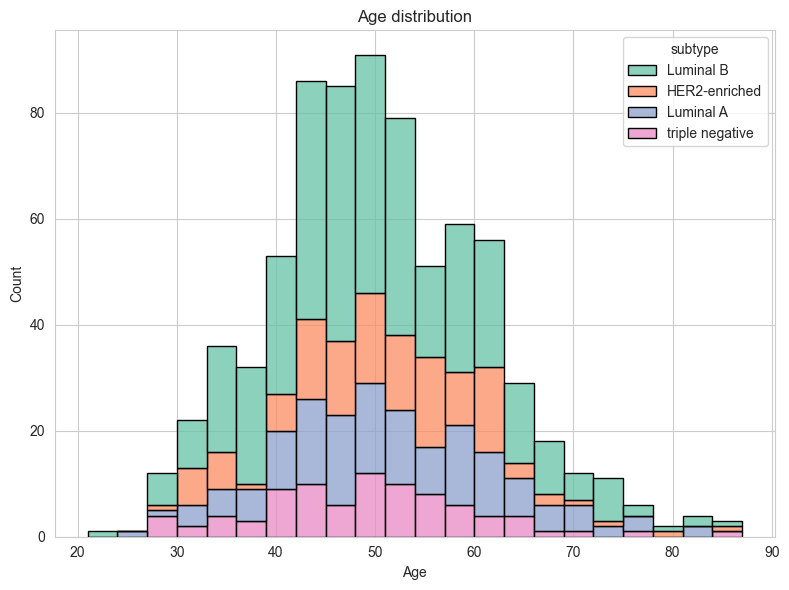
\includegraphics[width=\textwidth]{reports/assets/age_subtype.png}
		\caption{Age and subtype distribution}
		\label{fig:age_subtype}
	\end{subfigure}
	\caption[CMMD2 Age distribution]{(a) Overall age distribution of patients and (b) distribution by cancer subtype (CMMD2).}
	\label{fig:age_dist_all}
\end{figure}

Figure \ref{fig:age_dist_all} illustrates both the overall age distribution and the age distribution stratified by molecular subtype.

The analysis of molecular subtype distribution within the CMMD2 dataset is also crucial, as it determines the statistical representativeness of each class and consequently affects the models' generalization capability in clinical scenarios. The dataset exhibits significant class imbalance\footnote{Class imbalance refers to unequal representation of different classes in a dataset, where some classes have substantially more or fewer samples than others.}, with Luminal B being the most prevalent subtype (376 patients, 50.2\%), followed by Luminal A (152 patients, 20.3\%), HER2-enriched (135 patients, 18.0\%), and Triple Negative as the least represented subtype (86 patients, 11.5\%).

The class imbalance is also reflected in the total number of images available per subtype, as each patient contributes at least two mammographic views (CC and MLO projections), with few exceptions. This imbalance presents a significant challenge for machine learning classification models, which tend to exhibit bias toward majority classes when appropriate balancing strategies are not implemented. Nevertheless, this distribution accurately reflects the relative prevalence observed in clinical practice, where Luminal subtypes (A and B) are most common, while Triple Negative breast cancer represents approximately 10-15\% of all cases.

\begin{figure}[h!]
	\centering
	\begin{subfigure}[c]{0.45\textwidth}
		\centering
		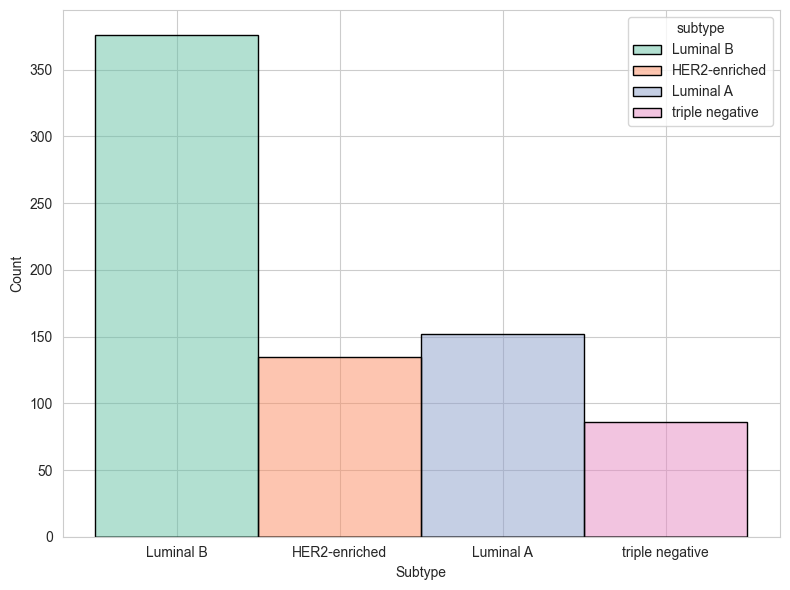
\includegraphics[width=\textwidth]{reports//assets/subtype_hist.png}
		\caption{Subtype distribution}
		\label{fig:subtype_hist}
	\end{subfigure}
	\begin{subfigure}[c]{0.45\textwidth}
		\centering
		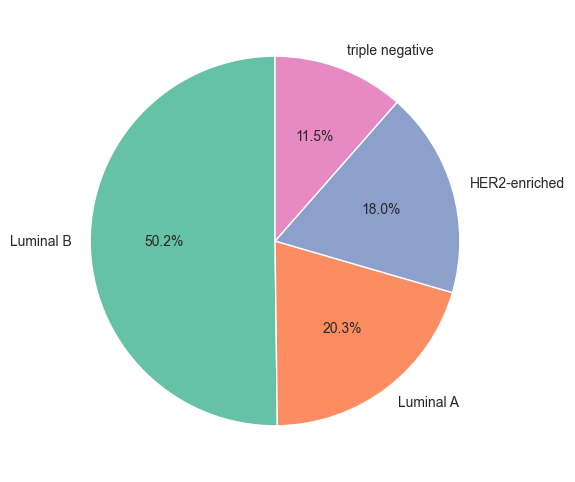
\includegraphics[width=\textwidth]{reports/assets/subtype_pie.png}
		\caption{Subtype distribution (pie chart)}
		\label{fig:subtype_pie}
	\end{subfigure}
	\caption[CMMD2 molecular subtypes distribution]{Subtype distribution of patients (CMMD2)}
	\label{fig:subtype_charts}
\end{figure}


\begin{figure}[h!]
	\centering
	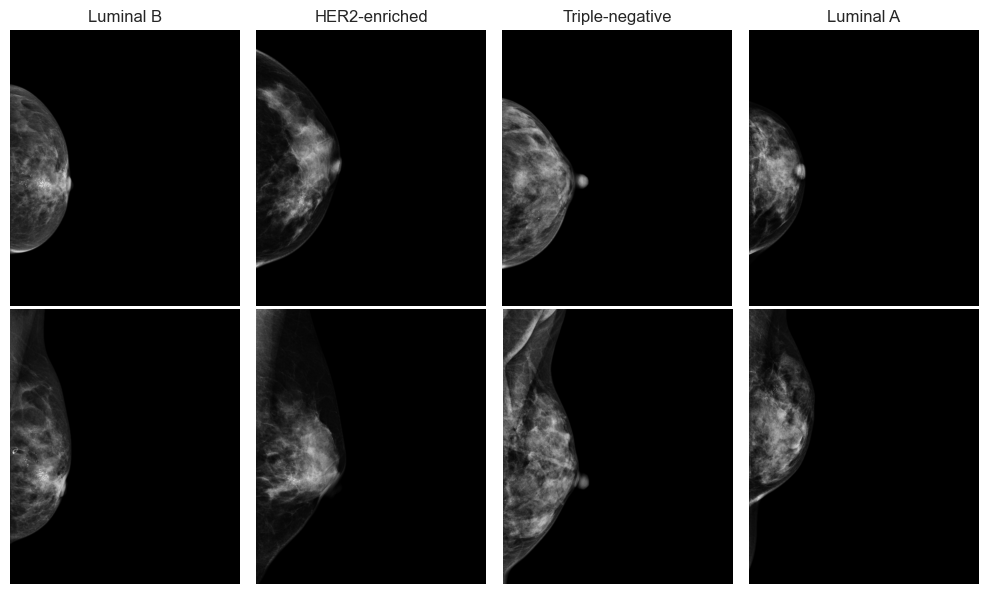
\includegraphics[width=1\linewidth]{reports//assets/images_examples.png}
	\caption[CMMD2 mammography images examples]{Example of mammography images of the CCMD2 dataset. Top row represent a CC view whereas bottom row illustrated a MLO view. Each column depicted one subtype of cancer.}
	\label{fig:cmmd-examples}
\end{figure}

\newpage
\section{The TOMPEI-CMMD review}

The TOMPEI-CMMD represents an enhanced version of the original CMMD, developed by Kashiwada et al. (2025) \cite{kashiwada_tompei-cmmd_2025}. This enhancement aimed to provide comprehensive radiological insights and perform a systematic re-evaluation of the existing mammographic images. A board-certified radiologist with 20 years of experience in breast imaging assessed all images, documenting detailed radiological findings including masses, calcifications, focal asymmetric densities, architectural distortions, and their anatomical locations. The dataset further provides pixel-level segmentation masks for all identified findings in MLO views, created following the radiologist's expert assessment. 

One of the most important results of the evaluation process was the exclusion of 140 breast images that did not meet the quality and diagnostic criteria. 

\section{Image Preprocessing}


\section{Data splitting and stratification strategy}
\section{Development tools}
\section{Evaluation Metrics}
\section{Experiments}

\chapter{Results and Discussion}
\chapter{Conclusions and Future Work}

\chapter{Appendix A}

%%%%%%%%%%%%%%%%%%%%%%%%%%%%%%%%%%%%%%%%%%%%%%%%%%%%%%%%%%%%%%%%%%%%%%%%%
\backmatter
\selectlanguage{english}
\addcontentsline{toc}{chapter}{Bibliography}
\bibliographystyle{IEEEtran}
\bibliography{references}

\end{document}